\chapter{Проектирование модели системы}
\label{cha:chap4}

\section{Математическая модель двигателя}

Трёх фазный БДПТ может быть описан следующей системой уравнений\cite{art:dtc_smo}: 
\begin{align}
\label{sys:abc}
\left\{ \begin{aligned} 
  v_{ab}=R_si_{ab}+L_s\dfrac{d}{dt}i_{ab}+e_{ab}\\
  v_{bc}=R_si_{bc}+L_s\dfrac{d}{dt}i_{bc}+e_{bc}\\
  v_{ca}=R_si_{ca}+L_s\dfrac{d}{dt}i_{ca}+e_{ca}
\end{aligned} \right.
\end{align}, где $a$, $b$, $c$ --- фазы двигателя; $v_{ab}$, $v_{bc}$, $v_{ca}$ --- напряжения между соответствующими фазами; $i_{ab}$, $i_{bc}$, $i_{ca}$ --- разница токов соответствующих фаз; $e_{ab}$, $e_{bc}$, $e_{ca}$ --- противо-ЭДС между соответствующими фазами; $R_s$ --- сопротивление статора; $L_s$ --- индуктивность статора

Уравнение динамики описывается следующим образом:
\begin{align*}
	T_e = T_L+B\omega_m+J\dfrac{d\omega_m}{dt}
\end{align*}, где $T_e$ --- электромагнитный момент; $T_L$ --- момент нагрузки; $B$ --- коэффициент трения; $J$ --- момент инерции ротора; $\omega_m$ --- механический момент ротора

Противо-ЭДС может быть выражена следующей зависимостью от скорости:
\begin{align*}
	e_{abc}=k_e\omega_m
\end{align*}, где $k_e$ --- постоянная по противо-ЭДС

\section{Наблюдатель скользящего режима (SMO)}
\label{sec:smo}

Т. к. у нас двигатель без установленных датчиков положения, то нам необходимо его оценивать для реализации алгоритма управления. Можно рассмотреть классический наблюдатель Люенбергера \cite{art:obs_luen_bldc}, но его устойчивость сильно зависит от параметров, используемых при построении, что не подходит под требования технического задания. Поэтому был выбран наблюдатель на основе скользящего режима, т. к. он работает при вариации параметров двигателя во время работы, т. е. обладает большей рабостностью. Также он требует меньше вычислительных мощностей, что позволяет увеличить частоту измерений.

Для удобства дальнейших расчётов запишем \ref{sys:abc} в двумерной $\alpha-\beta$ системе:
\begin{align}
\label{sys:albet}
\left\{ \begin{aligned} 
  &v_{\alpha}=R_si_{\alpha}+L_s\dfrac{d}{dt}i_{\alpha}+e_{\alpha}\\
  &v_{\beta}=R_si_{\beta}+L_s\dfrac{d}{dt}i_{\beta}+e_{\beta}
\end{aligned} \right.
\end{align}

Или в матричной форме: \cite{art:smo}
\begin{align}
\label{sys:albetmat}
\dot{i}_{\alpha\beta}=\Phi i_{\alpha\beta}+\Gamma v_{\alpha\beta}-\Gamma e_{\alpha\beta}
\end{align}, где $i_{\alpha\beta}=\begin{bmatrix}
	i_{\alpha} & i_{\beta}
\end{bmatrix}$, $v_{\alpha\beta}=\begin{bmatrix}
	v_{\alpha} & v_{\beta}
\end{bmatrix}$, $e_{\alpha\beta}=\begin{bmatrix}
	e_{\alpha} & e_{\beta}
\end{bmatrix}$, $\Phi=\begin{bmatrix}
	-R_s/L_s & 0 \\
	0 & -R_s/L_s
\end{bmatrix}$, $\Gamma = \begin{bmatrix}
	1/L_s & 0 \\
	0 & 1/L_s
\end{bmatrix}$

Также поведение противо-ЭДС может быть представлено в следующей форме:
\begin{align}
\label{e_albet}
	\dot{e}_{\alpha\beta}=\omega_eJe_{\alpha\beta}
\end{align}, где $\omega_e$ --- электрическая скорость двигателя ($\omega_e=\omega_m\cdot p$ ($p$ --- количество пар полюсов двигателя)); $J=\begin{bmatrix}
 0 & -1 \\
 1 & 0
\end{bmatrix}$

Рассмотрим дискретный наблюдатель, рассмотренный в \cite{art:smo}. Для этого рассмотрим \ref{sys:albetmat} и \ref{e_albet} в дискретной форме:
\begin{align}
	&i_{\alpha\beta(k+1)}=Ai_{\alpha\beta(k)}+Bv_{\alpha\beta(k)}-Be_{\alpha\beta(k)}\\
	&e_{\alpha\beta(k+1)}=e_{\alpha\beta(k)}+T_s\omega_{e(k)}Je_{\alpha\beta(k)}
\end{align}, где $T_s$ --- период дискретизации; $A=e^{\Phi T_s}$; $B=\int_0^{T_s}e^{\Phi\tau}\Gamma d\tau=\begin{bmatrix}
	b & 0 \\
	0 & b
\end{bmatrix}$ $\left(b=\dfrac{1-e^{-R_sT_s/L_s}}{R_s}\right)$

Тогда наблюдатель на основе скользящего режима задаётся следующими уравнениями:
\begin{align}
	&\hat{i}_{\alpha\beta(k+1)}=A\hat{i}_{\alpha\beta(k)}+Bv_{\alpha\beta(k)}-B\hat{e}_{\alpha\beta(k)}-\eta sign(\tilde{i}_{\alpha\beta(k)})\\
	\label{eq:hat_e}
	&\hat{e}_{\alpha\beta(k+1)}=\hat{e}_{\alpha\beta(k)}+B^{-1}g(\tilde{i}_{\alpha\beta(k)}-A\tilde{i}_{\alpha\beta(k-1)}+\eta sign(\tilde{i}_{\alpha\beta(k-1)}))\\
	&\tilde{i}_{\alpha\beta(k)}=\hat{i}_{\alpha\beta(k)}-i_{\alpha\beta(k)}\\
	&\tilde{e}_{\alpha\beta(k)}=\hat{e_{\alpha\beta(k)}}-e_{\alpha\beta(k)}
\end{align}, где $\eta$ --- коэффициент усиления по противо-ЭДС; $g$ --- коэффициент усиления по току

Выбор коэффициентов осуществляется из следующих условий:
\begin{enumerate}
	\item Если $|e_{\alpha\beta(k+1)}-e_{\alpha\beta(k)}|\leq m$ и коэффициент $g\in (0, 1)$ тогда существует $k_0$ такое, что при $k\geq k_0$ выполняется:
	\begin{align*}
		\tilde{e}_{\alpha\beta(k)}<\dfrac{m}{g}
	\end{align*}
	\item Если $|e_{\alpha\beta(k+1)}-e_{\alpha\beta(k)}|\leq m$, коэффициент $g\in (0, 1)$ и $\eta>b\dfrac{m}{g}$ тогда существует $k_0$ такое, что при $k\geq k_0$ выполняется:
	\begin{align*}
		|\tilde{i}_{\alpha\beta(k)}|\leq \eta +b\dfrac{m}{g}
	\end{align*}
\end{enumerate}

Таким образом, при правильном выборе параметров наблюдателя обеспечивается ограниченность векторов невязки по противо-ЭДС и току.

Главным недостатком такого вида наблюдателя, как и любых систем на основе скользящих режимов, является чаттеринг (дребезг) при приближении к поверхности скольжения, что уменьшает точность регулирования и увеличивает частоту перключений фаз, внося дополнительные потери и понижая срок службы электрических компонентов. Для уменьшения его амплитуды может применяться фильтр нижних частот на выходе оценок противо-ЭДС \cite{art:smo} и/или замена функций знакового переключения на функции переключения с насыщением \cite{art:dtc_smo}.

Оценка электрического положение ротора может быть найдено из \ref{eq:hat_e} по следующей формуле:
\begin{align*}
	\hat{\theta}_e = \tan^{-1}\left(-\dfrac{\hat{e_\alpha}}{\hat{e_\beta}}\right)
\end{align*}

Из чего можно найти скорость вращения ротора, зная число пар полюсов двигателя ($p$).

\section{Прямое управление моментом}

Для реализации этого алгоритма управления необходимо знание электромагнитного момента ($T_e$), который может быть найден следующим образом\cite{art:dtc_smo}:  
\begin{align}
	\label{Te}
	&T_e=\dfrac{3p}{4}\left(\dfrac{d\Psi_{r\alpha}}{d\theta_e}i_{\alpha}+\dfrac{d\Psi_{r\beta}}{d\theta_e}i_{\beta}\right)
\end{align}, где $\Psi_{r\alpha}$, $\Psi_{r\beta}$ --- поток статора в $\alpha-\beta$ координатах.

Производные потока ротора от электрического положения ротора могут быть представлены следующими соотношениями:
\begin{align}
	\label{psira}
	&\dfrac{d\Psi_{r\alpha}}{d\theta_e}=\dfrac{d\Psi_{r\alpha}}{dt}\dfrac{dt}{d\theta_e}=\dfrac{1}{\omega_e}\dfrac{d\Psi_{r\alpha}}{dt}=\dfrac{e_\alpha}{\omega_e}\\
	&\dfrac{d\Psi_{r\beta}}{d\theta_e}=\dfrac{d\Psi_{r\beta}}{dt}\dfrac{dt}{d\theta_e}=\dfrac{1}{\omega_e}\dfrac{d\Psi_{r\beta}}{dt}=\dfrac{e_\beta}{\omega_e}
\end{align}

С учётом \ref{psira} и \ref{Te} можем получить:
\begin{align*}
	T_e=\dfrac{3p}{4}\left(\dfrac{e_{\alpha}}{\omega_e}i_{\alpha}+\dfrac{e_{\beta}}{\omega_e}i_{\beta}\right)
\end{align*}

Из этого уравнения и оценки противо-ЭДС рассчитывается значения оценки электромагнитного момента:
\begin{align}
\label{eq:T_e}
	&\hat{T}_e=\dfrac{3p}{4}\left(\dfrac{\hat{e}_{\alpha}}{\omega_e}i_{\alpha}+\dfrac{\hat{e}_{\beta}}{\omega_e}i_{\beta}\right)=\dfrac{3}{4}\left(\dfrac{\hat{e}_{\alpha}}{\omega_m}i_{\alpha}+\dfrac{\hat{e}_{\beta}}{\omega_m}i_{\beta}\right)
\end{align}

В нашей системе мы будем управлять только моментом, не затрагивая управление потоком для уменьшения вычислительных затрат и возможности дополнительно повысить период дискретизации.

\section{Модель системы в Simulink}

На основе математических формул, приведённых выше, была построена модель системы, приведённая на рисунке \ref{pic:mod1}.

\begin{figure}[!h]
\centering
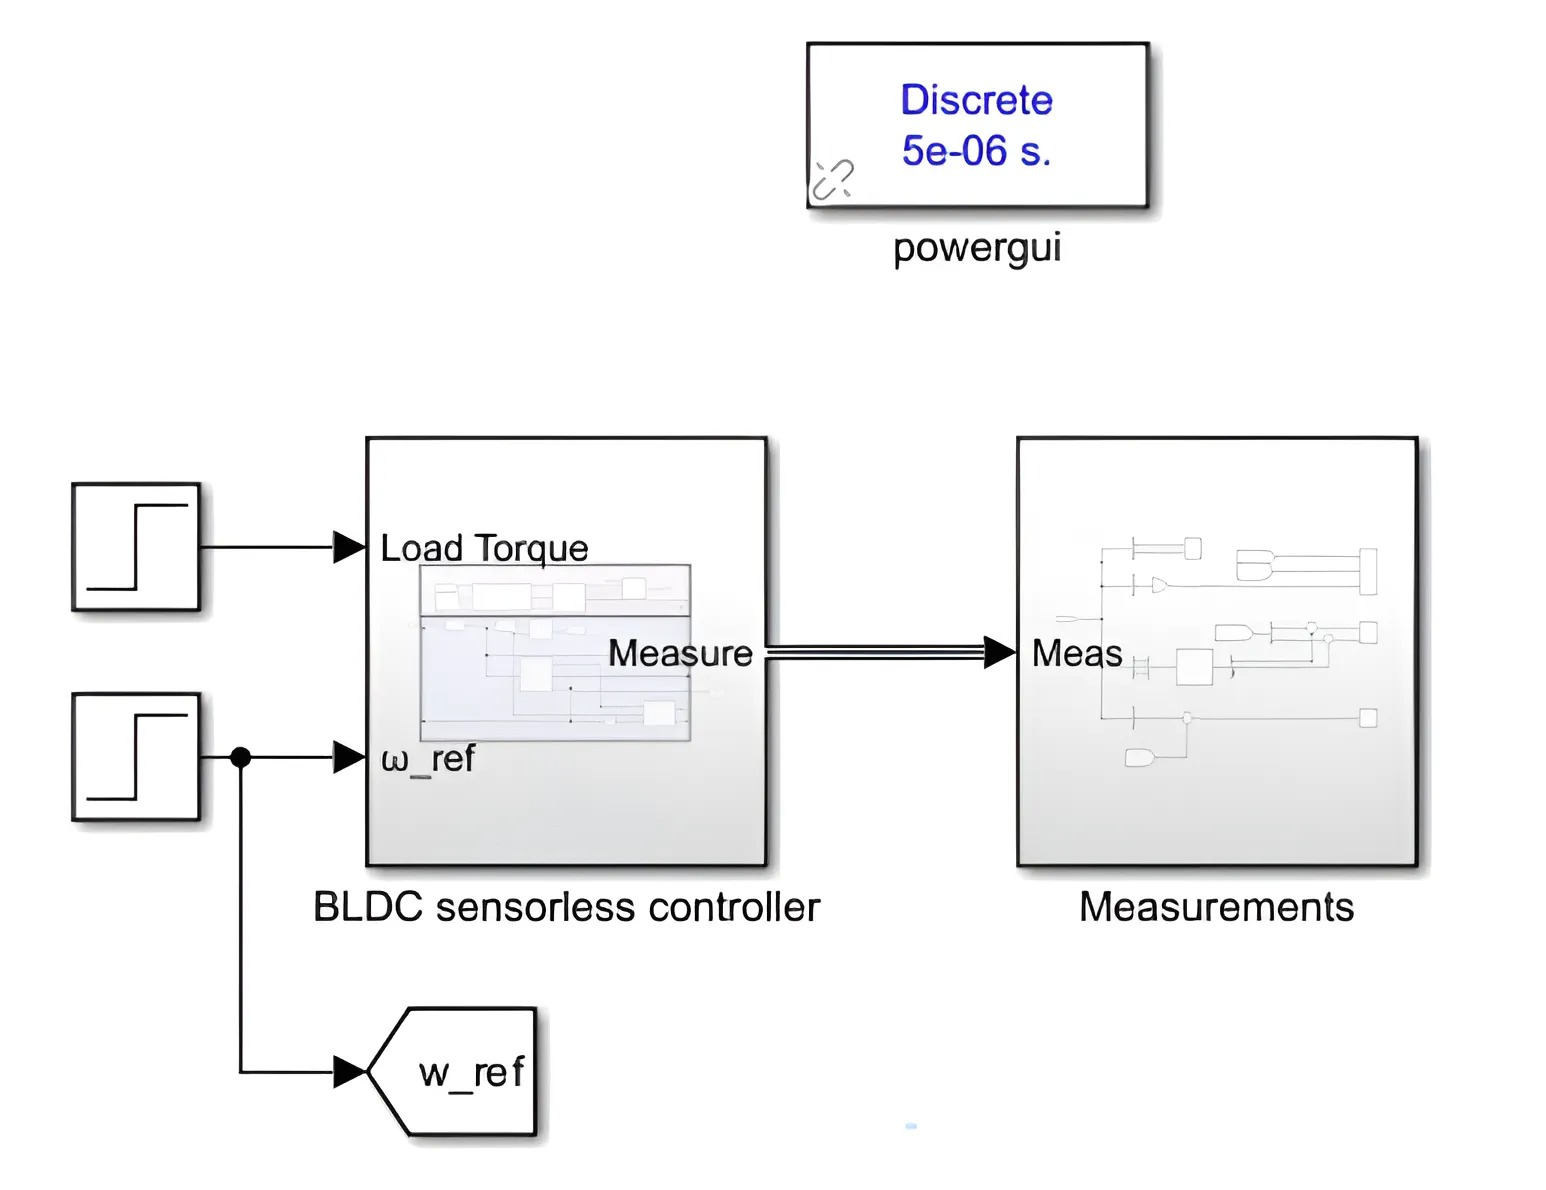
\includegraphics[width=0.7\textwidth]{inc/img/model1.png}
\caption{Общая модель системы}
\label{pic:mod1}
\end{figure}

Она состоит из двух основных блоков. Первый из них приведён на рисунке \ref{pic:mod2} и содержит силовую часть из инвертора, двигателя и источника питания, систему управления, которая представляет из себя двухконтурный регулятор (первый контур по скорости, второй по моменту). Электромагнитный момент находится по формуле \ref{eq:T_e} на основе параметров, получаемых при оценке с помощью наблюдателя скользящего режима, описанного в \ref{sec:smo}.

\begin{figure}[!h]
\centering
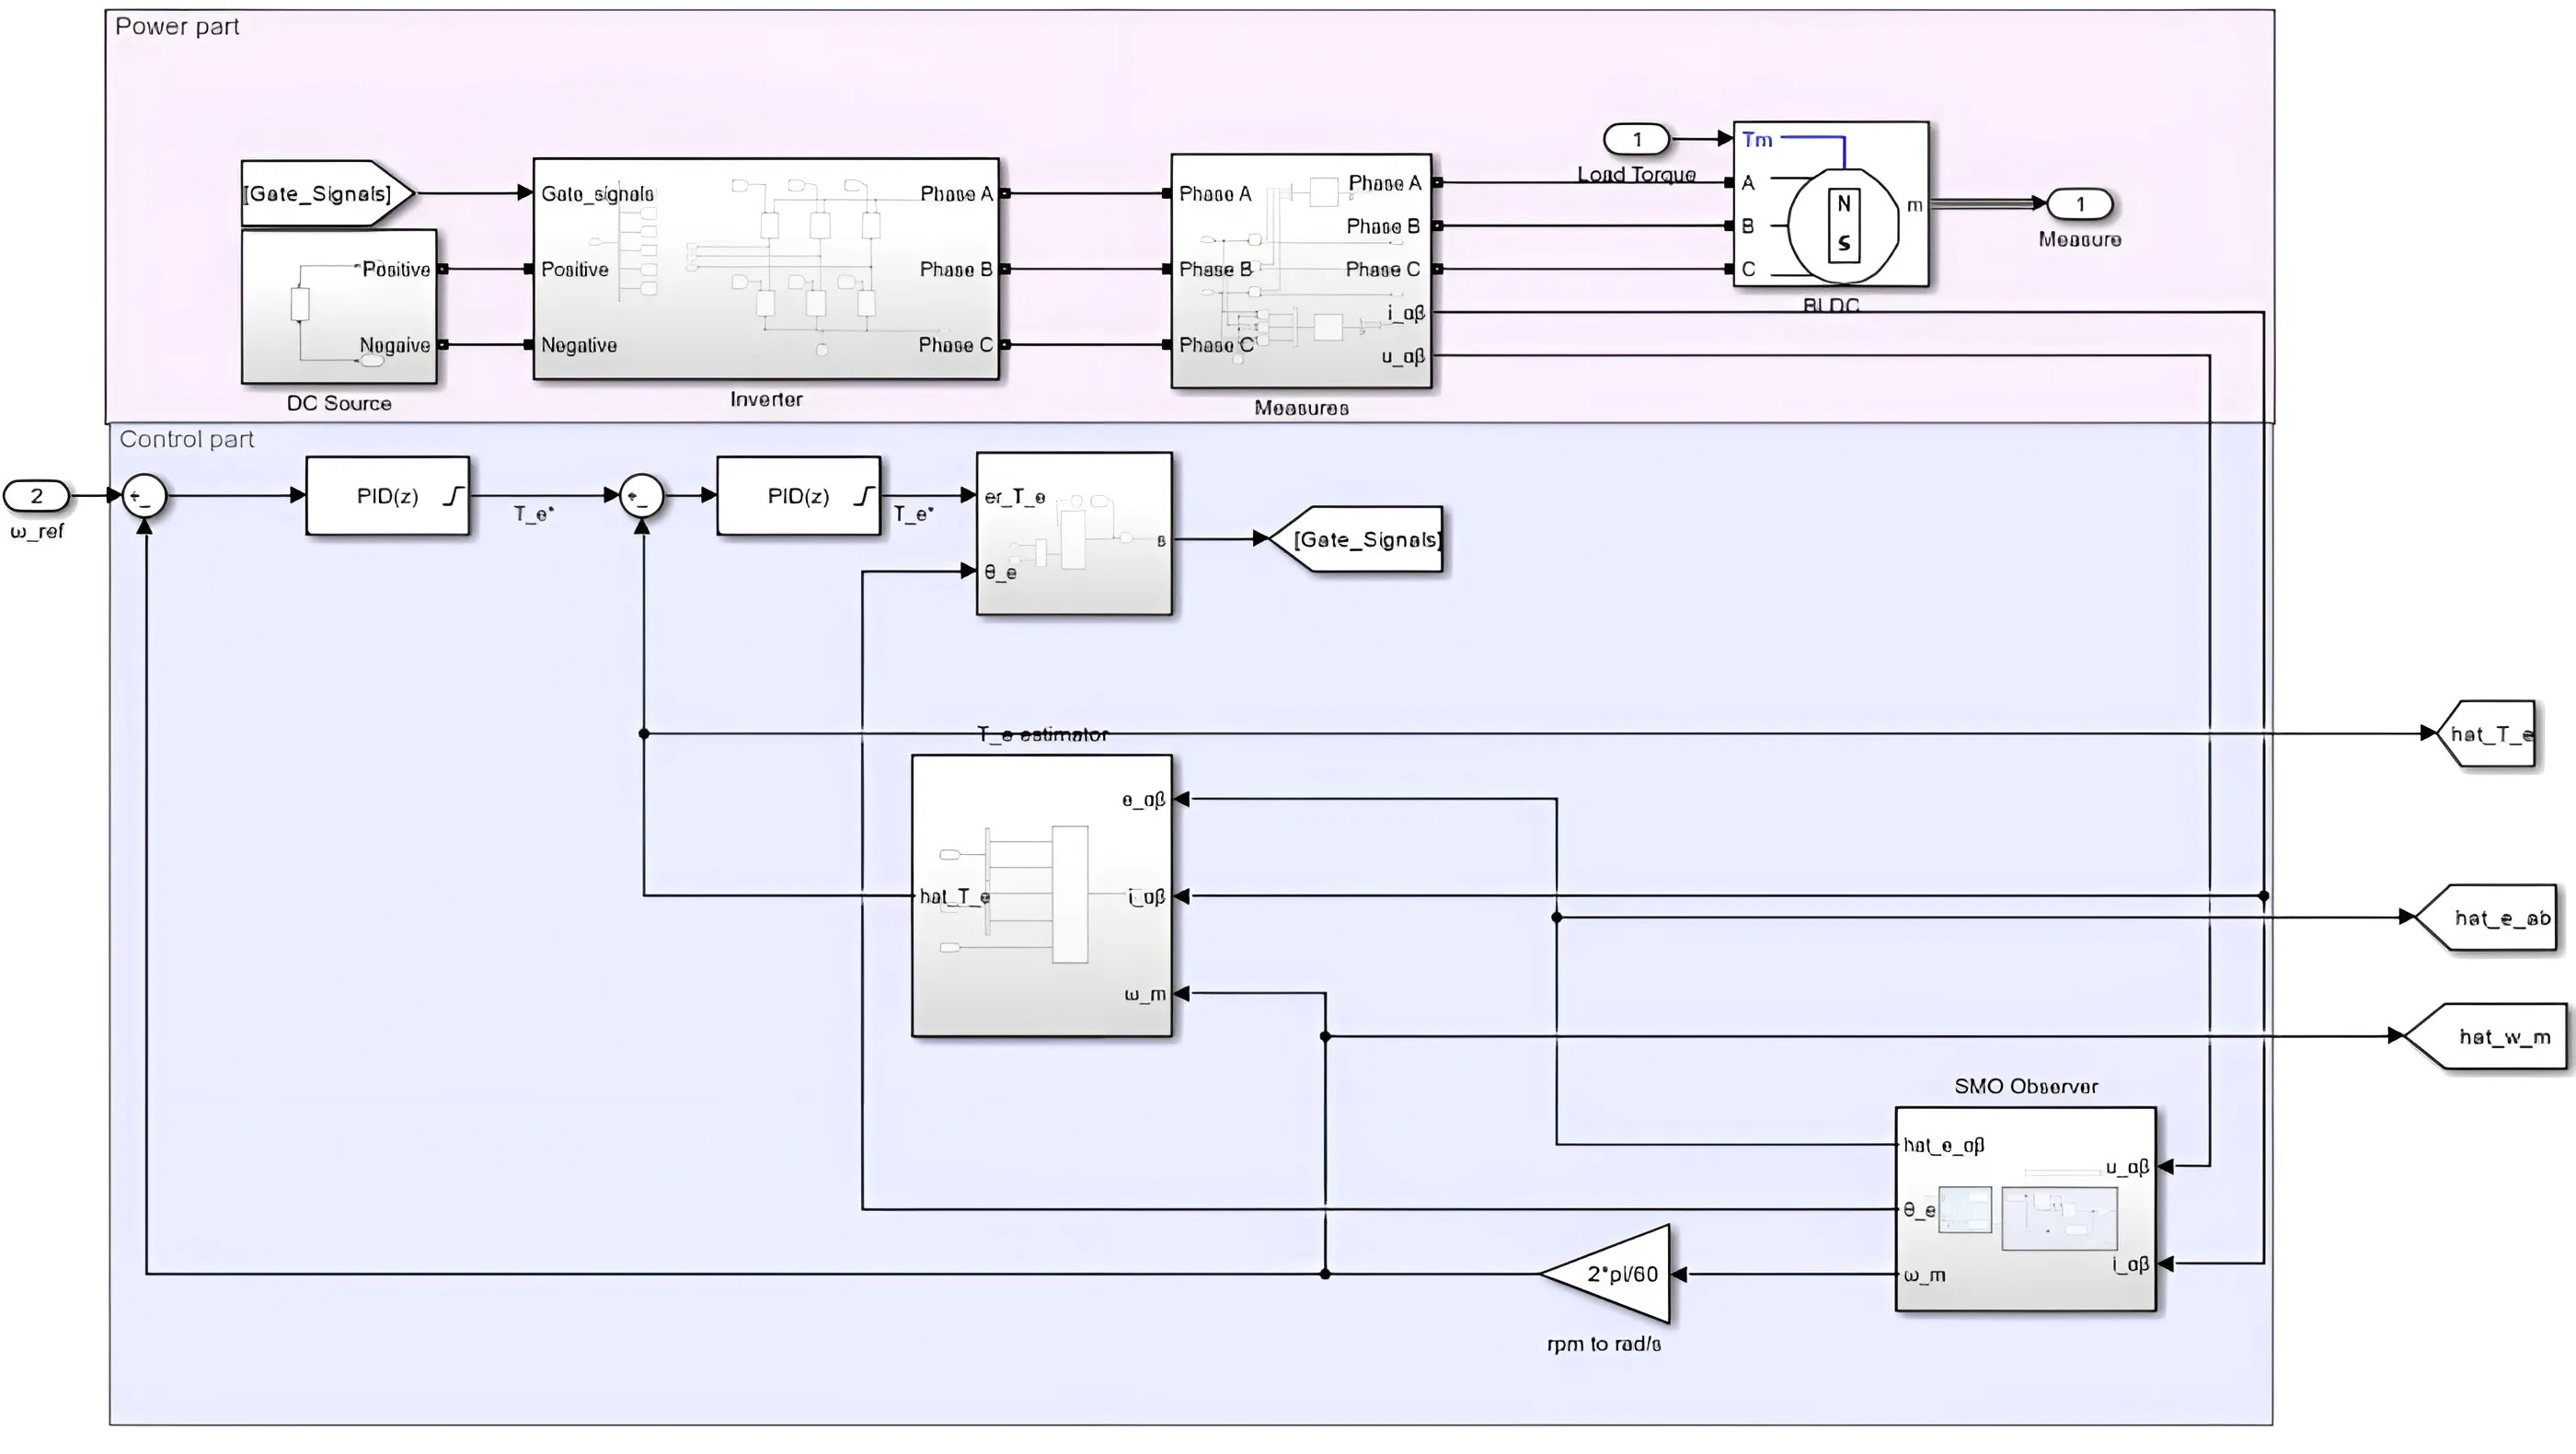
\includegraphics[width=1\textwidth]{inc/img/model2.png}
\caption{Блок с системой управления и силовой частью}
\label{pic:mod2}
\end{figure}

Инвертор представляет собой 6 ключей на основе Mosfet транзисторов (Рисунок \ref{pic:mod4}) и питается от источника постоянного напряжения (Рисунок \ref{pic:mod3})

\begin{figure}[!h]
\centering
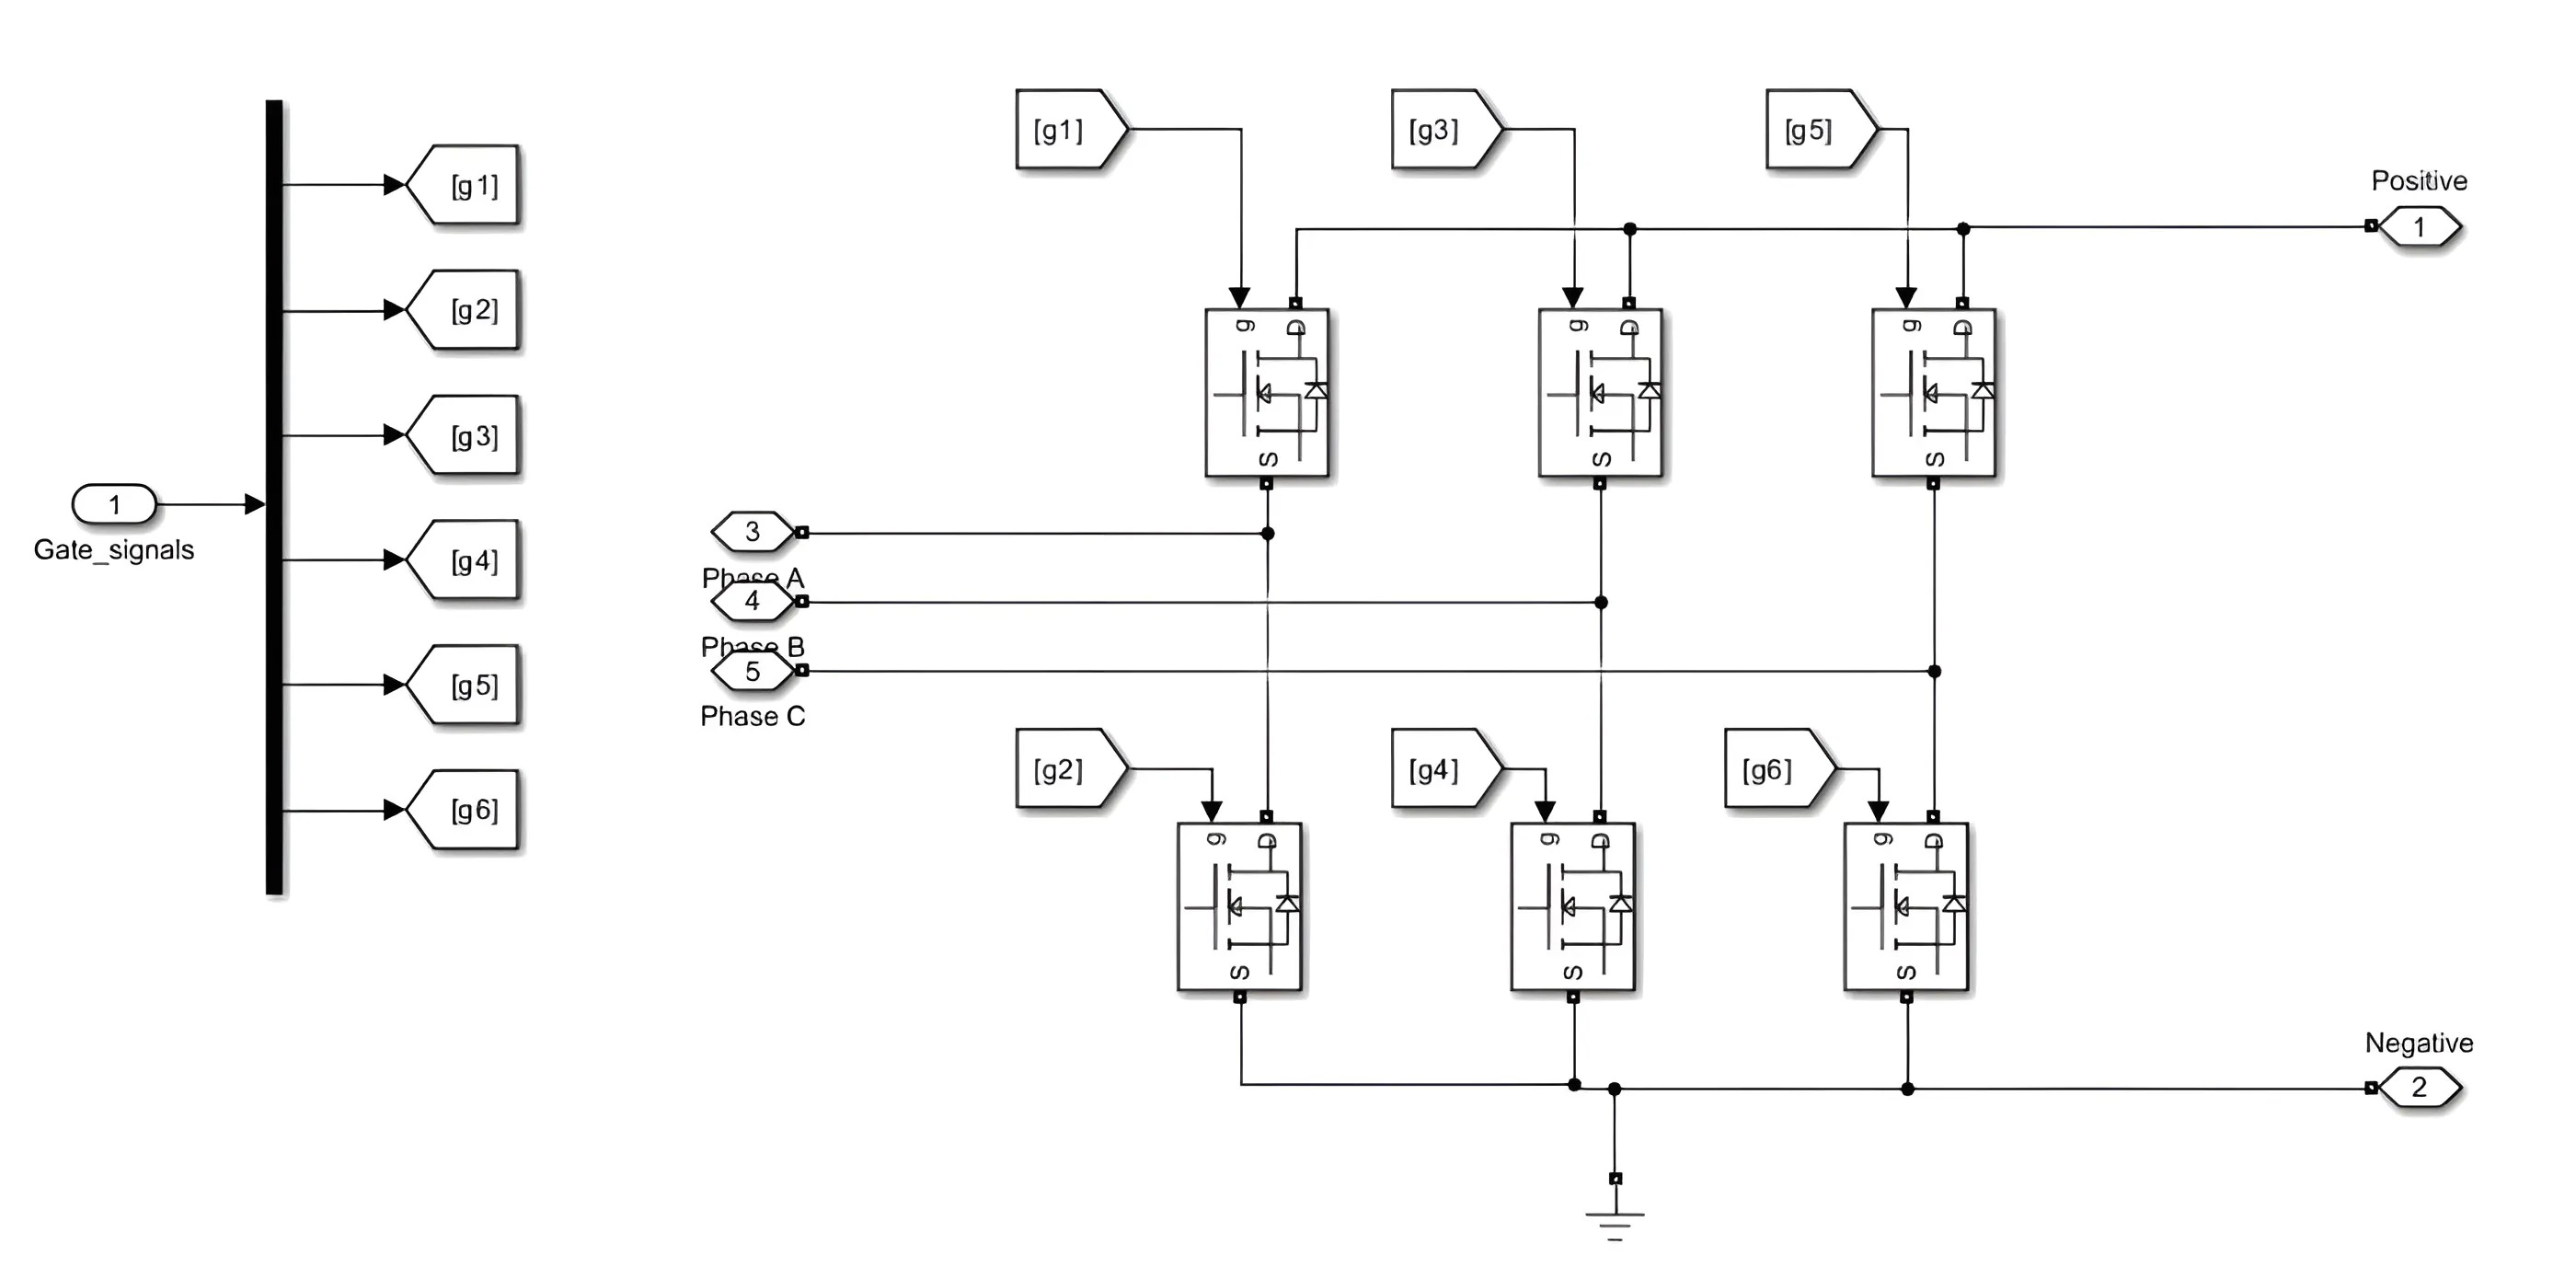
\includegraphics[width=1\textwidth]{inc/img/model4.png}
\caption{Трёхфазный инвертор}
\label{pic:mod4}
\end{figure}

\begin{figure}[!h]
\centering
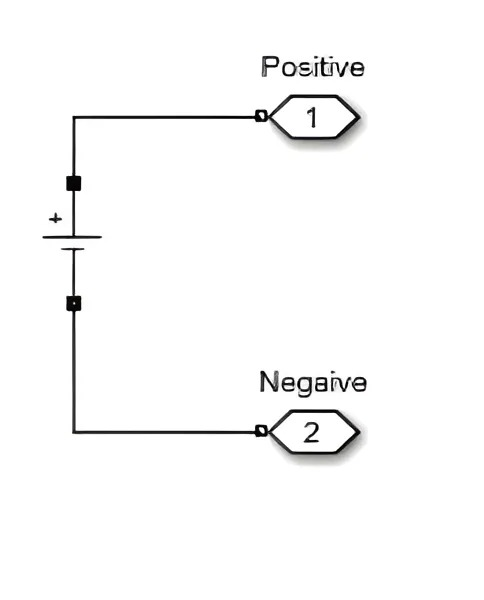
\includegraphics[width=0.3\textwidth]{inc/img/model3.png}
\caption{Источник постоянного тока}
\label{pic:mod3}
\end{figure}

Переключение ключей происходит по текущему электрическому положению ротора с использованием ШИМ, скважность которого регулируется в зависимости от модуля значения выхода значения, получаемого на выходе ПИ регулятора контура момента, выход которого ограничен диапазоном от $-1$ до $1$ (Рисунок \ref{pic:mod7}).

\begin{figure}[!h]
\centering
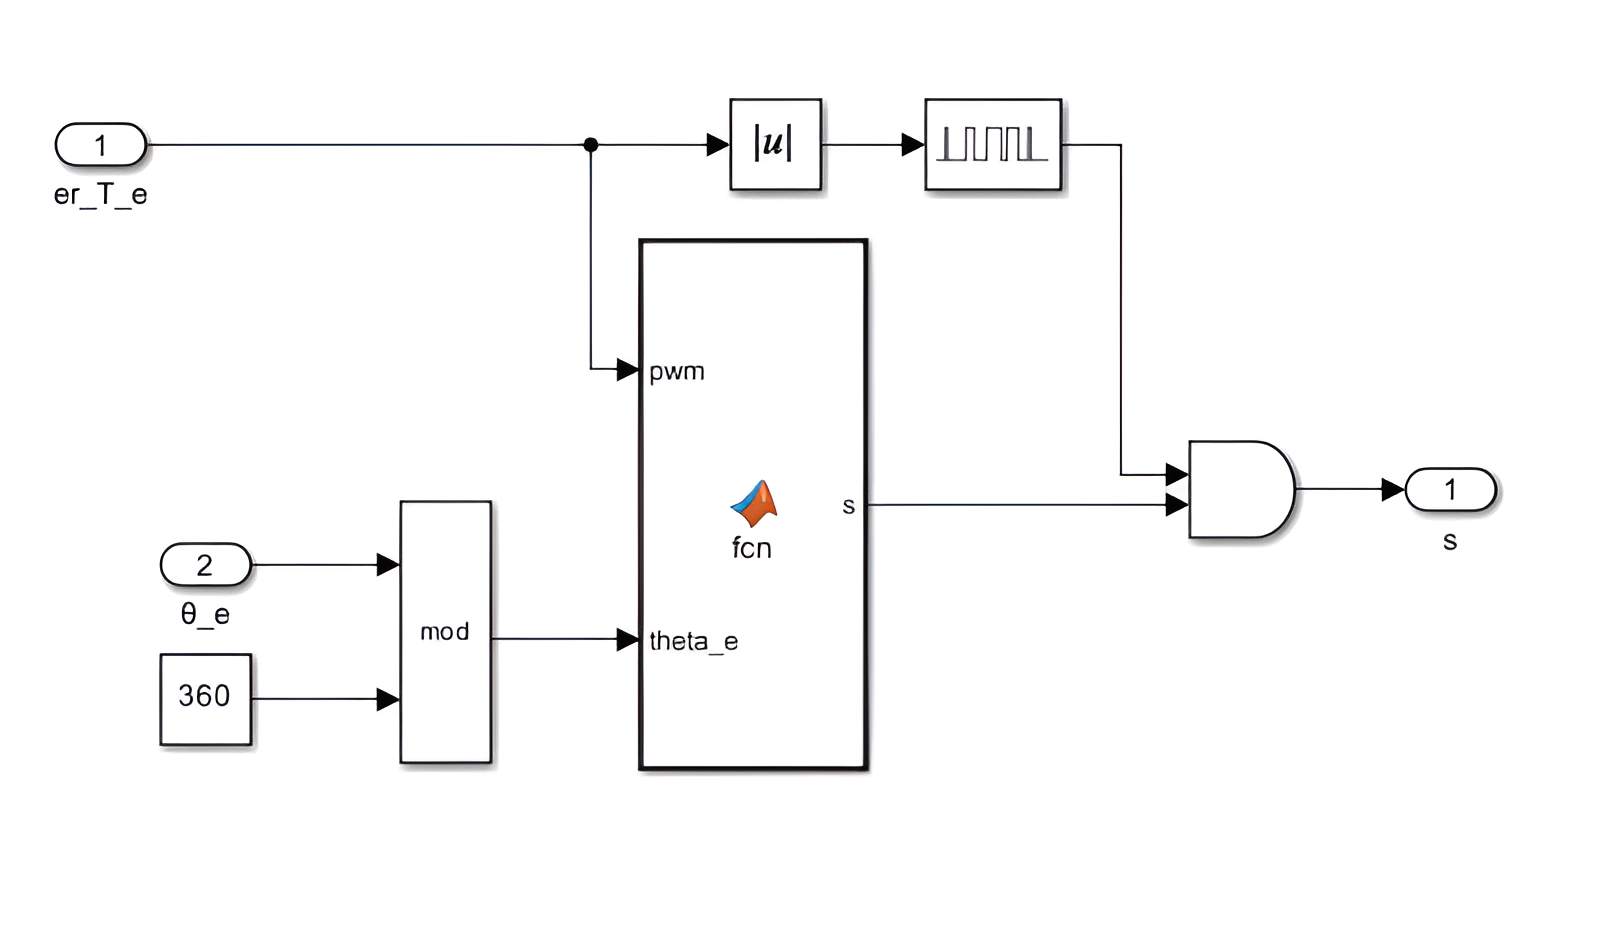
\includegraphics[width=0.7\textwidth]{inc/img/model7.png}
\caption{Система переключения ключей инвертора}
\label{pic:mod7}
\end{figure}

Возможные состояния в $\alpha-\beta$ системе с состояниями ключей приведены на Рисунке \ref{pic:vectors_dtc} и таблица коммутации в зависимости от электрического положения ротора и выхода ПИ регулятора момента приведены в Таблице \ref{table:com_dtc}.

\begin{figure}[!h]
\centering
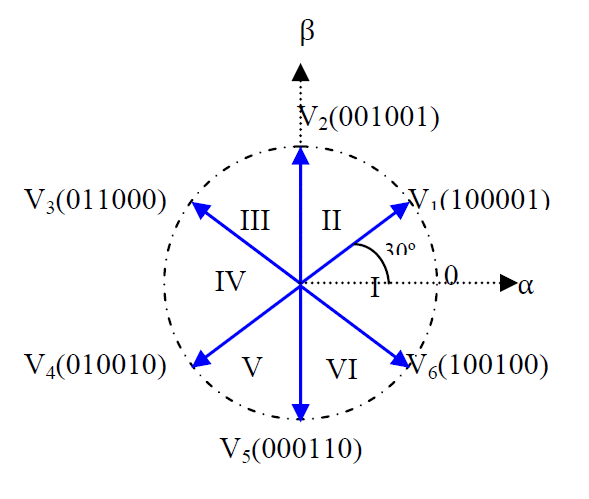
\includegraphics[width=0.7\textwidth]{inc/img/dtc_vectors.png}
\caption{Векторы переключения и состояния ключей \cite{art:dtc_smo}}
\label{pic:vectors_dtc}
\end{figure}

\begin{center}
\captionof{table}{схема коммутации от выхода регулятора\label{table:com_dtc}}
\begin{tabular}{|c|p{1.5cm}|p{1.5cm}|p{1.5cm}|p{1.5cm}|p{1.5cm}|p{1.5cm}|}
 \hline
 Выход ПИ регулятора & \multicolumn{6}{c|}{Электрическое положения ротора, $^\circ$} \\
 \hline
 [$0$---$1$] & $V_2$ & $V_3$ & $V_4$ & $V_5$ & $V_6$ & $V_1$ \\ 
 \hline
 [$-1$---$0$) & $V_5$ & $V_6$ & $V_1$ & $V_2$ & $V_3$ & $V_4$ \\
 \hline
\end{tabular}
\end{center}

\section{Результаты моделирования}
\label{sec:model_res}

Для моделирования использовались следующие параметры:
\begin{enumerate}
	\item Параметры двигателя (значения взяты от реального двигателя (\ref{sec:choose}), который будет использоваться в дальнейшем):
	\begin{align*}
		&R_s = 0,1\textrm{ Ом}\\
		&L_s = 0,0225\textrm{ Гн}\\
		&p = 4\\
		&k_e = 0,909\textrm{ B*мин/об}
	\end{align*}
	\item Параметры наблюдателя:
	\begin{align*}
		&g = 0,9\\
		&\eta = 7,8821e-4\\
		&f_{\textrm{среза}}=1200\textrm{ Гц}
	\end{align*}, где $f_{\textrm{среза}}$ --- частота среза для фильтра нижних частот на выходе оценки противо-ЭДС для уменьшения чаттеринга
	\item Параметры ПИ регулятора контура скорости:
	\begin{align*}
		&K_p = 2,39\\
		&K_i = 0,05
	\end{align*}
	\item Параметры ПИ регулятора контура момента:
	\begin{align*}
		&K_p = 0,01\\
		&K_i = 0,09
	\end{align*}\
	\item Частота дискретизации:
	\begin{align*}
		T = 1e-6\textrm{ с}
	\end{align*}
\end{enumerate}

Моделирования проводилось в трёх отрезках задачи скорости ($0-400$ рад/с, $400-600$ рад/с и $600-300$ рад/с) и каждый раз двигателю задавалось некоторая начальная скорость, ведь иначе при низких скоростях наблюдателю не получалось получить достаточно точную оценку противо-ЭДС для достижения желаемой скорости.

По техническому заданию нам не известны действительные значения сопротивления и индуктивности статора, известны лишь значения с погрешностью (в реальной работе двигателя эти параметры также могут варьироваться из-за нагрева двигателя в ходе работы, например, или других факторов), поэтому проводились моделирования также на граничных их значениях.

По результатам моделирования можно сказать, что вариация сопротивления практически не оказывает влияния на результаты работы наблюдателя и на переходные процессы в целом (Рисунки \ref{pic:R-}-\ref{pic:2R+}) в сравнении с эталонными параметрами (Рисунки \ref{pic:ideal} и \ref{pic:ideal2}), тогда как изменение индуктивности уменьшает скорость сходимости наблюдателя, что сказывается на времени переходного процесса и требует большего значения начальной скорости для достижения цели регулирования. Однако в пределах вариации параметров во всех экспериментах были выполнены требования, предъявляемые к алгоритму в техническом задании.

\begin{figure}[!h]
\centering
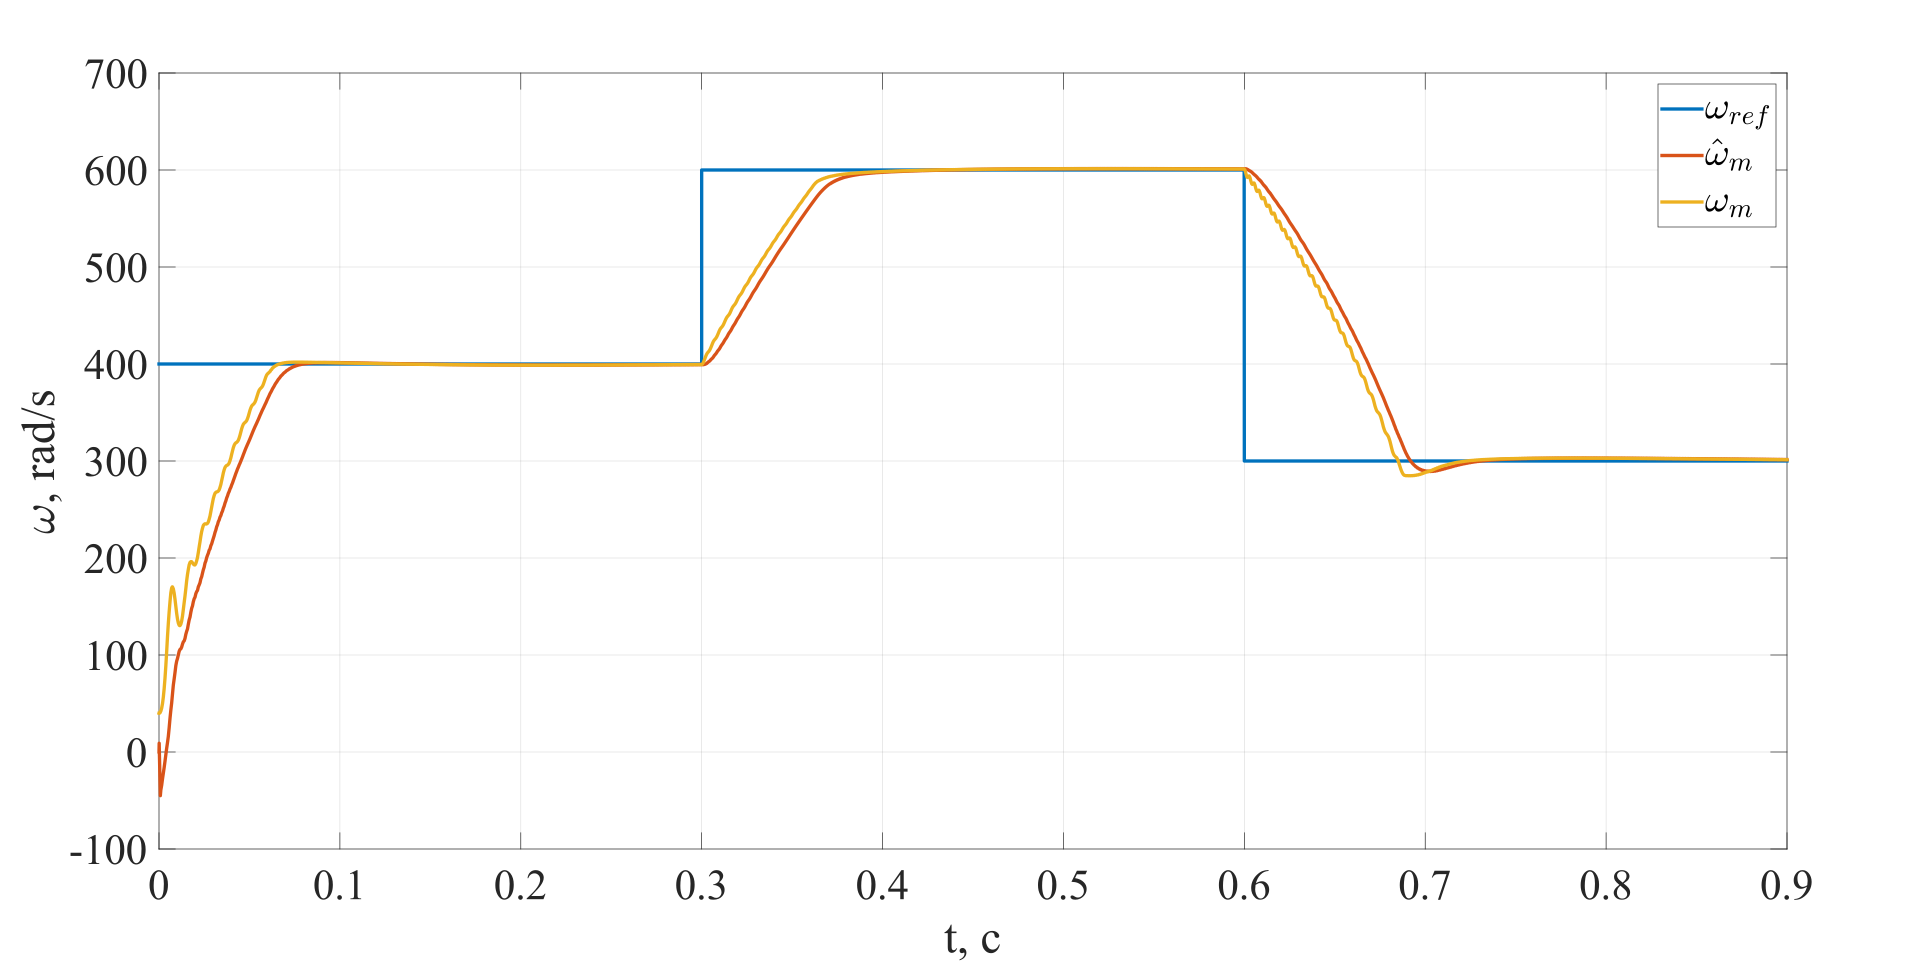
\includegraphics[width=\textwidth]{inc/svg/mod_resR}
\caption{Заданная, оцененная и действительная скорость ротора без вариации параметров}
\label{pic:ideal}
\end{figure}

\begin{figure}[!h]
\centering
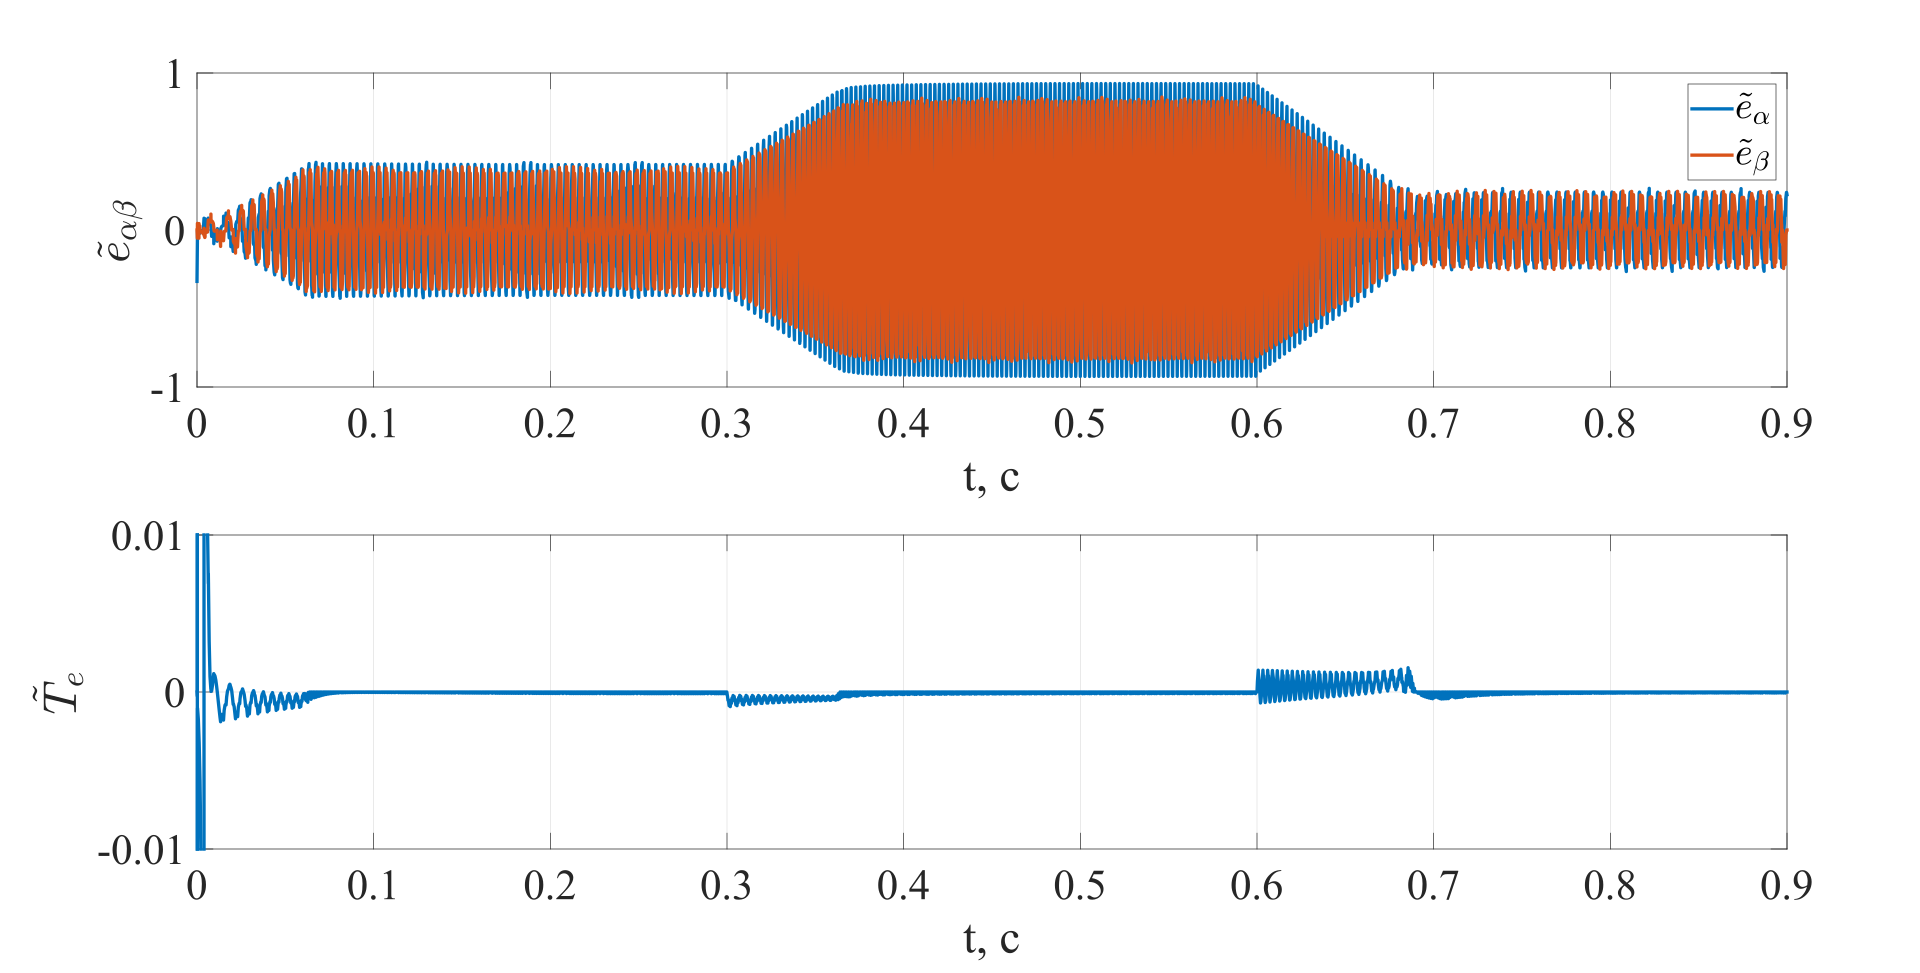
\includegraphics[width=\textwidth]{inc/svg/mod_res2R}
\caption{Вектор невязки по противо-ЭДС и электромагнитному моменту без вариации параметров}
\label{pic:ideal2}
\end{figure}

\begin{figure}[!h]
\centering
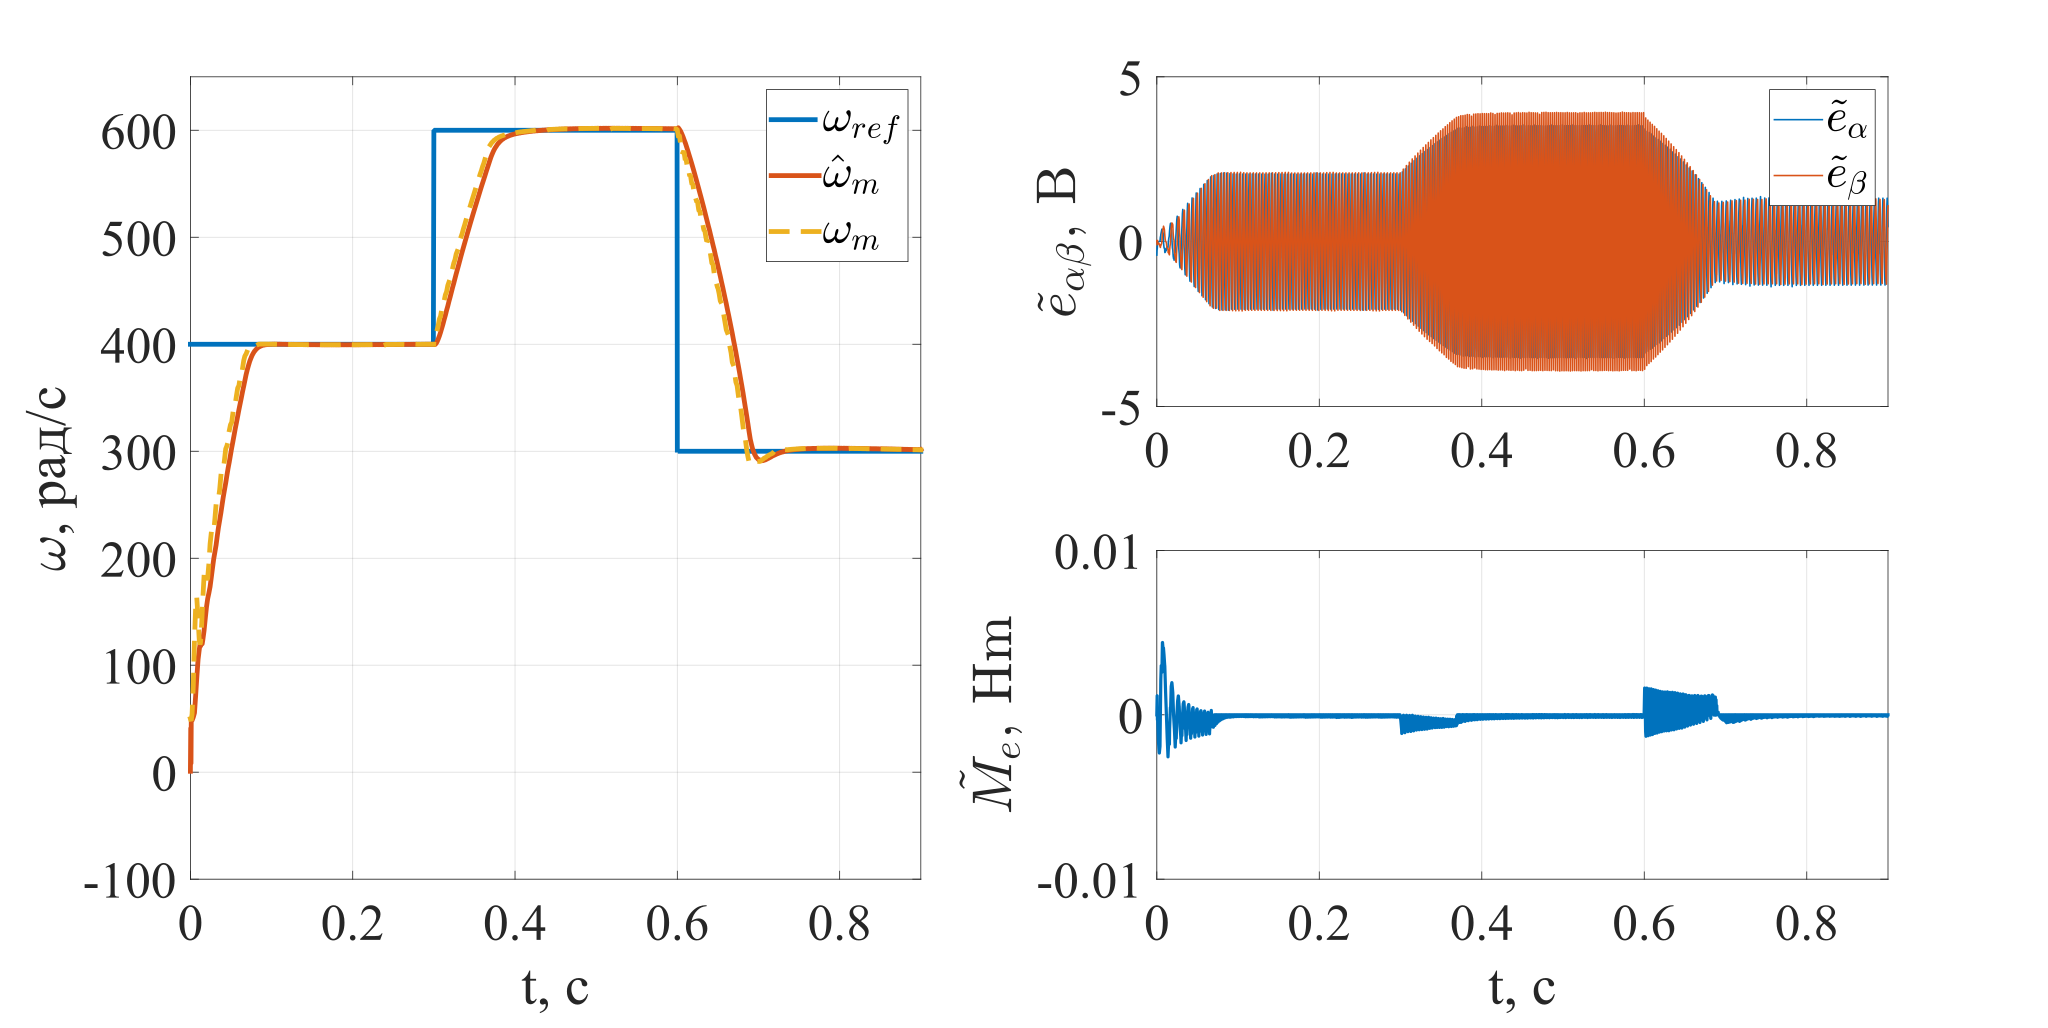
\includegraphics[width=\textwidth]{inc/svg/mod_resR-}
\caption{Заданная, оцененная и действительная скорость ротора при уменьшении $R$ на $100$ \%}
\label{pic:R-}
\end{figure}

\begin{figure}[!h]
\centering
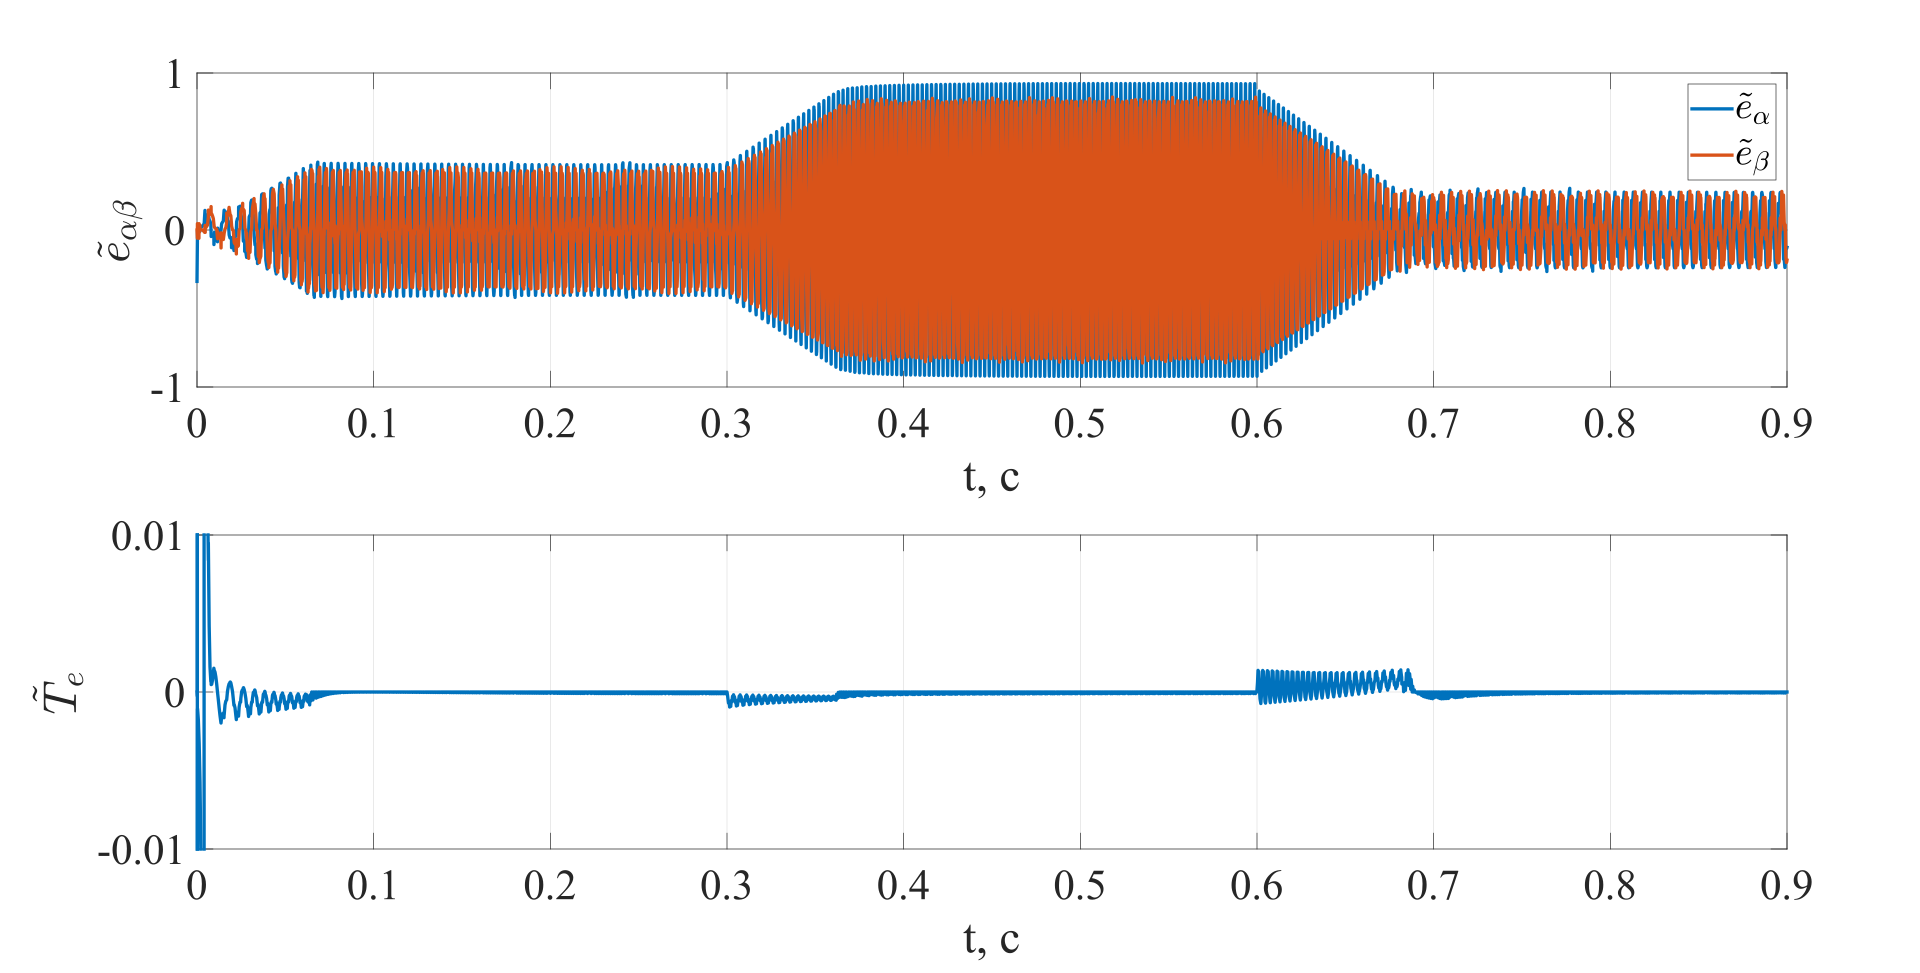
\includegraphics[width=\textwidth]{inc/svg/mod_res2R-}
\caption{Вектор невязки по противо-ЭДС и электромагнитному моменту при уменьшении $R$ на $100$ \%}
\label{pic:2R-}
\end{figure}

\begin{figure}[!h]
\centering
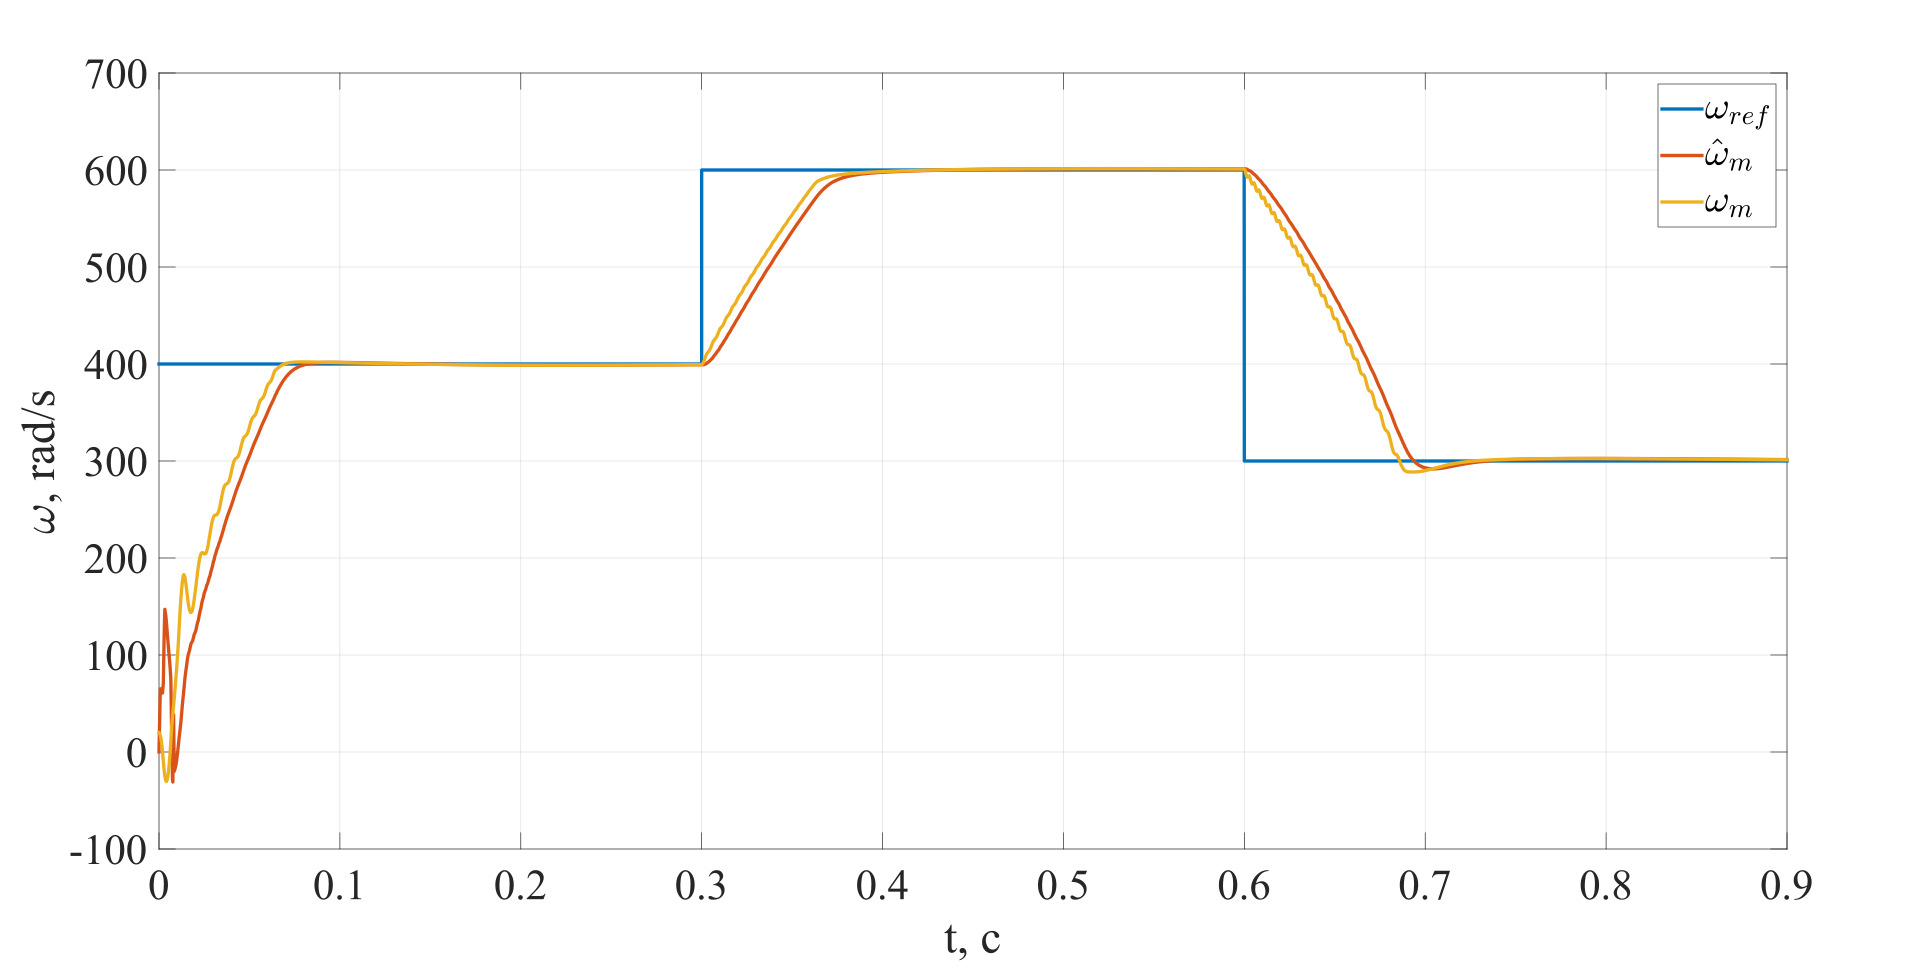
\includegraphics[width=\textwidth]{inc/svg/mod_resR+}
\caption{Заданная, оцененная и действительная скорость ротора при увеличении $R$ на $100$ \%}
\label{pic:R+}
\end{figure}

\begin{figure}[!h]
\centering
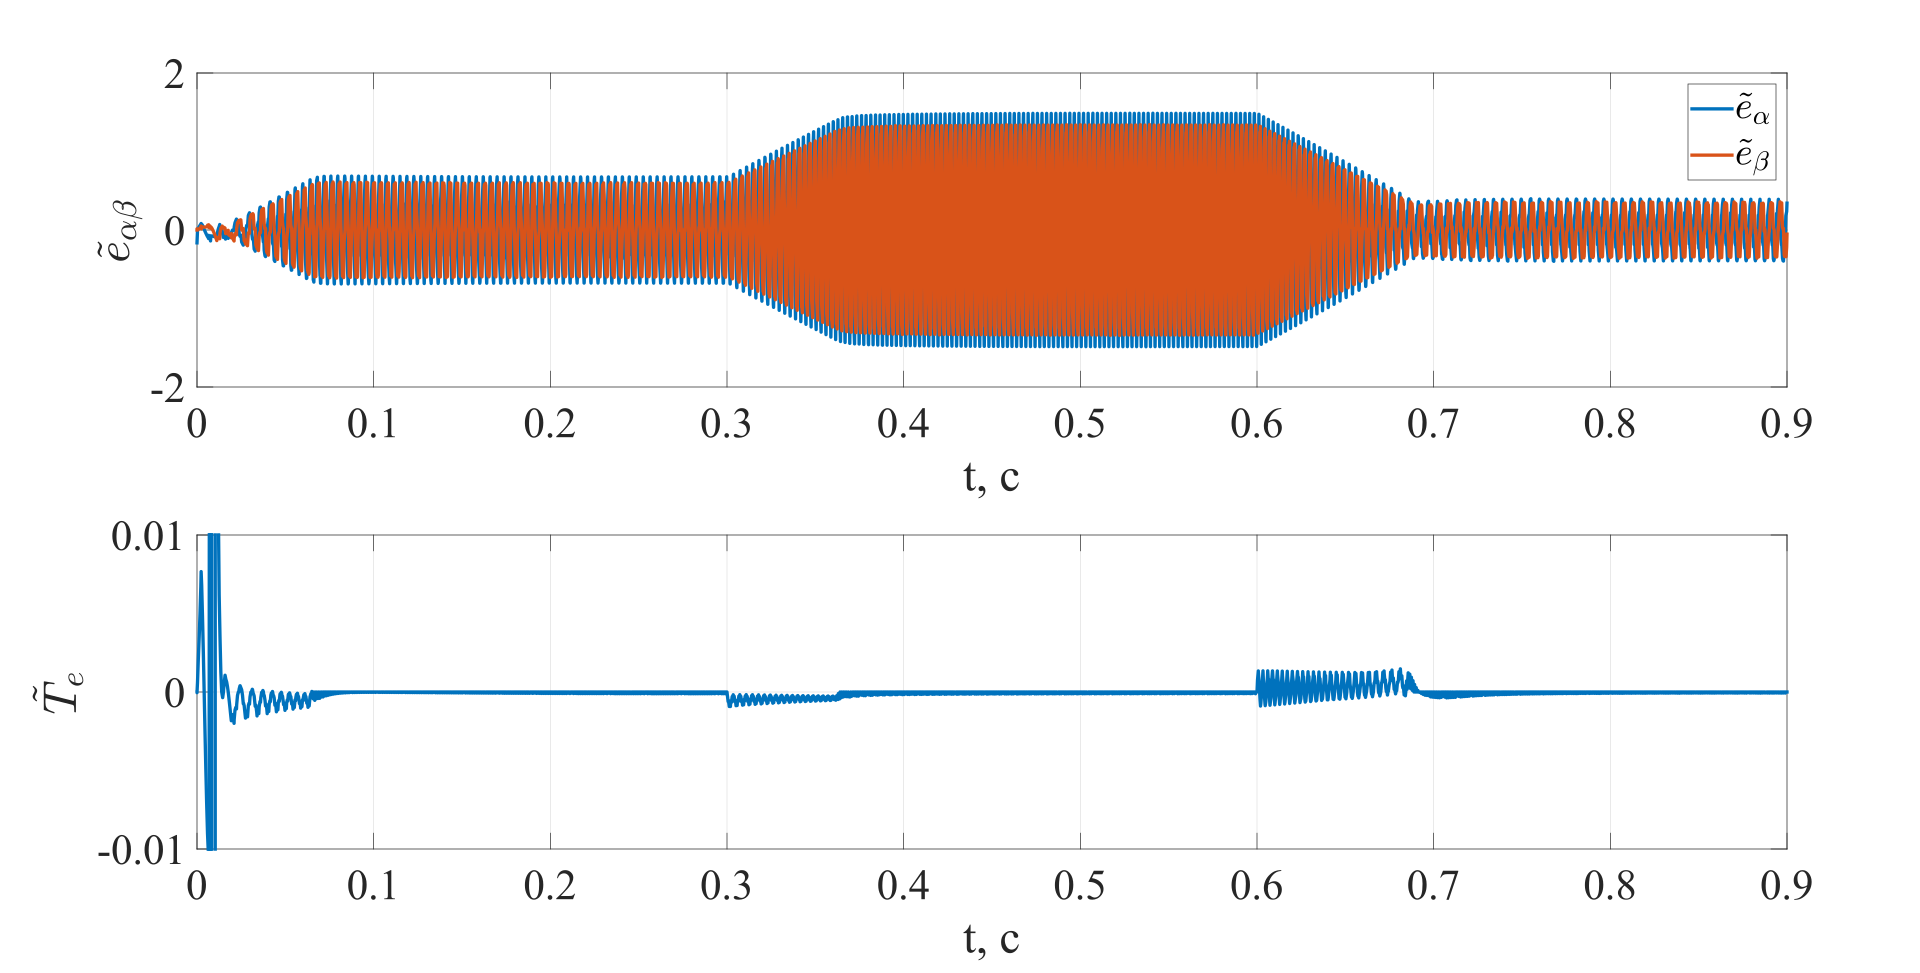
\includegraphics[width=\textwidth]{inc/svg/mod_res2R+}
\caption{Вектор невязки по противо-ЭДС и электромагнитному моменту при увеличении $R$ на $100$ \%}
\label{pic:2R+}
\end{figure}

\begin{figure}[!h]
\centering
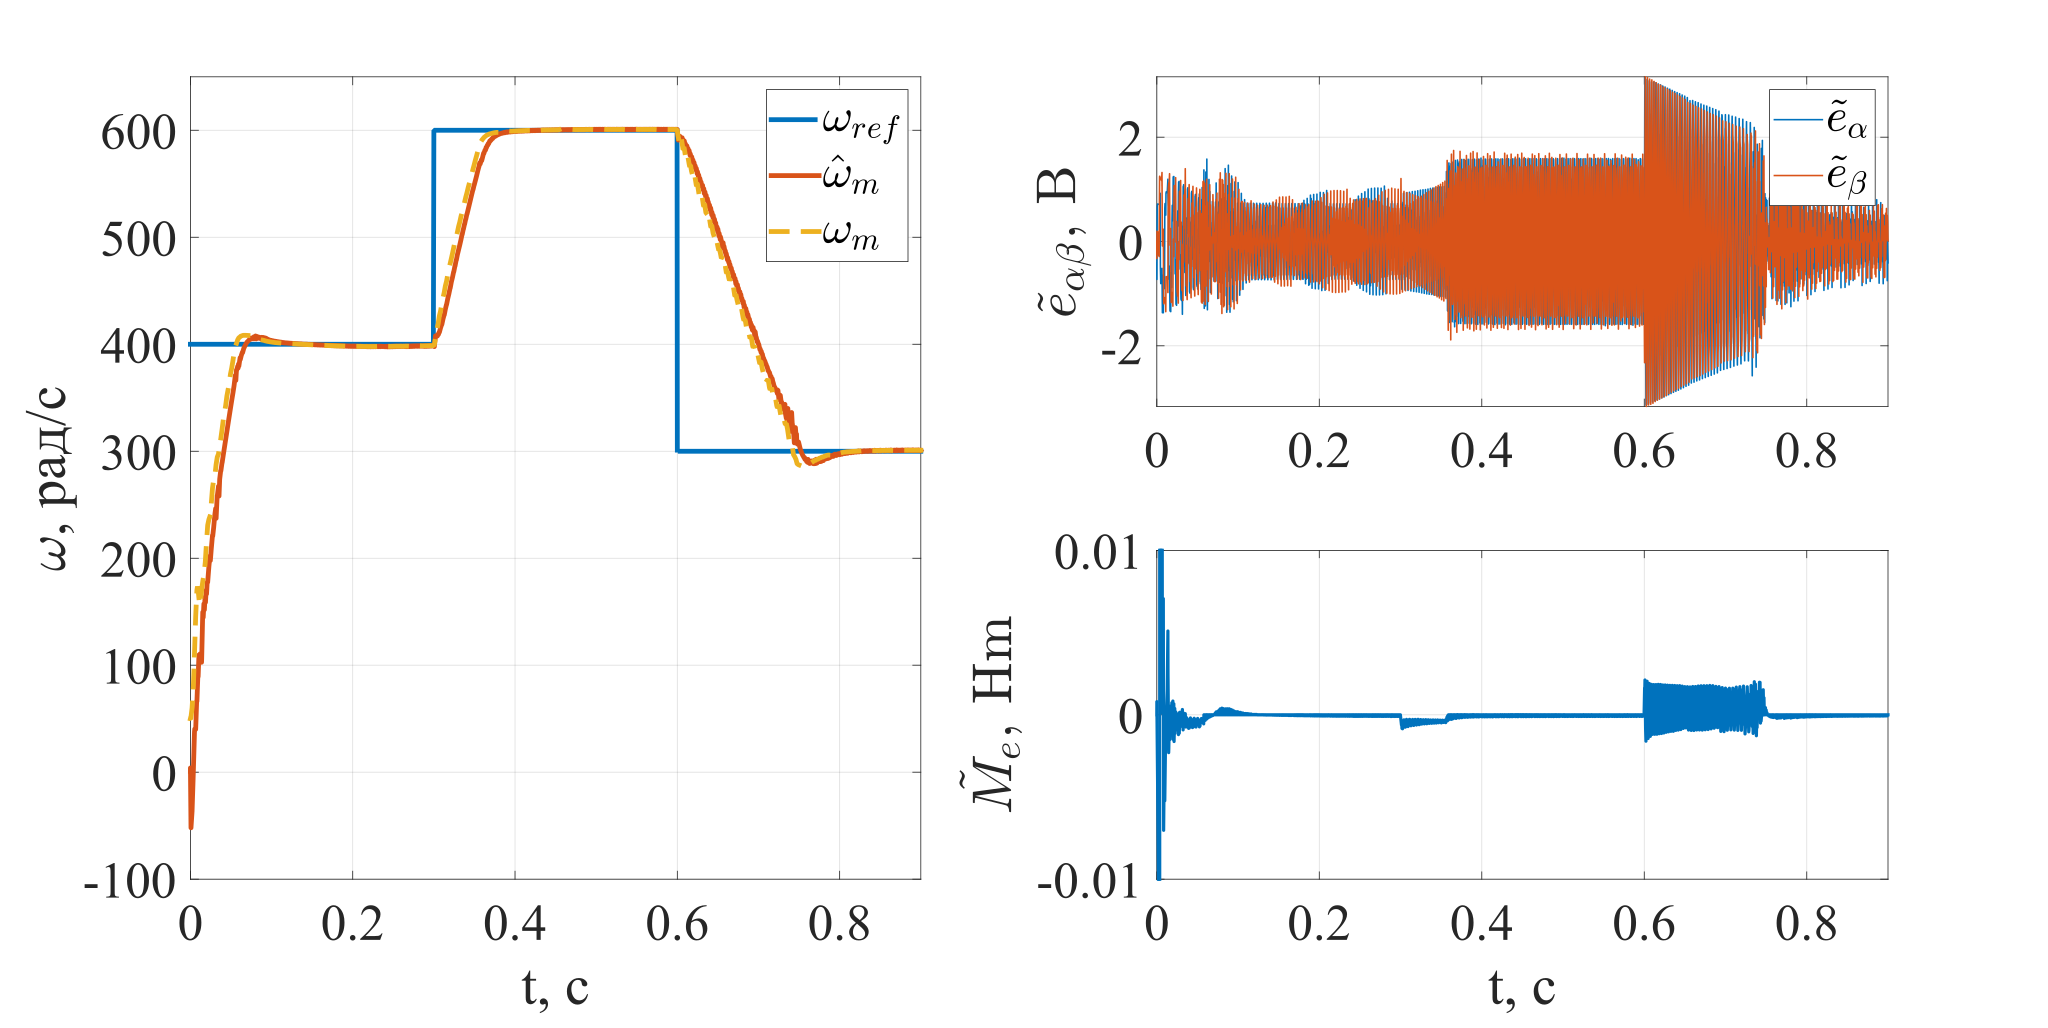
\includegraphics[width=\textwidth]{inc/svg/mod_resL-}
\caption{Заданная, оцененная и действительная скорость ротора при уменьшении $L$ на $10$ \%}
\label{pic:L-}
\end{figure}

\begin{figure}[!h]
\centering
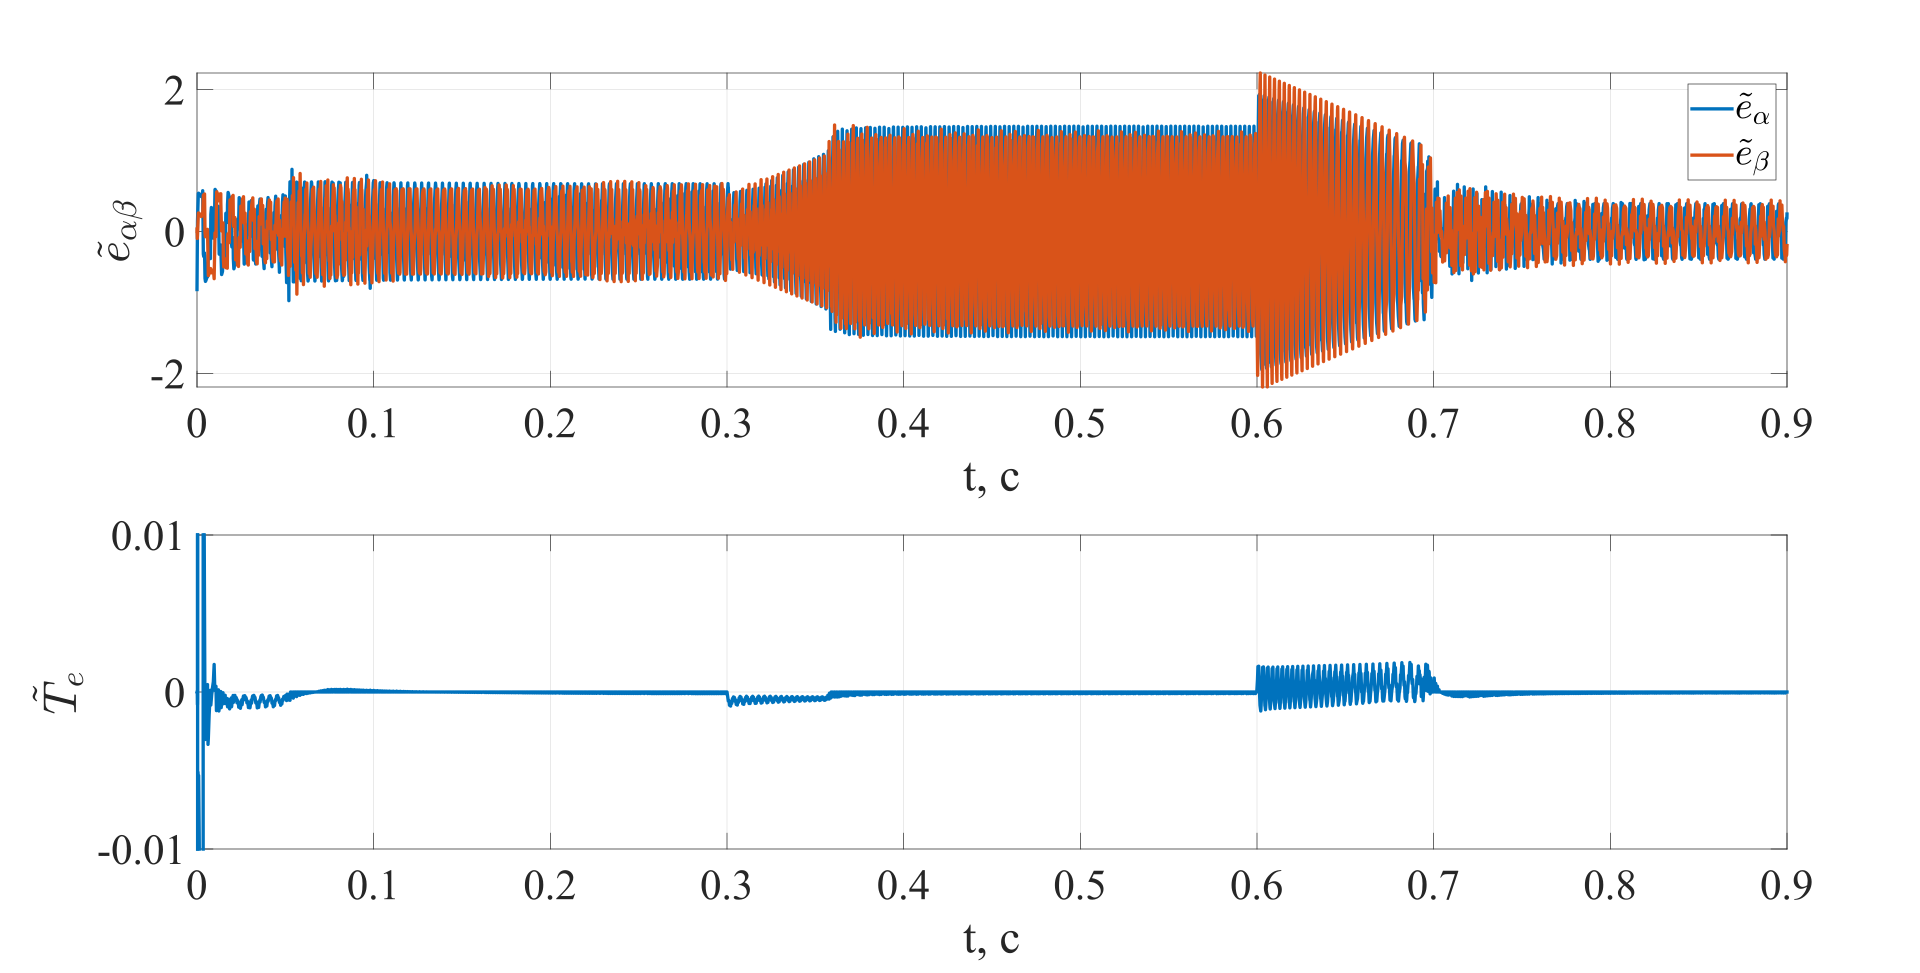
\includegraphics[width=\textwidth]{inc/svg/mod_res2L-}
\caption{Вектор невязки по противо-ЭДС и электромагнитному моменту при уменьшении $L$ на $10$ \%}
\label{pic:2L-}
\end{figure}

\begin{figure}[!h]
\centering
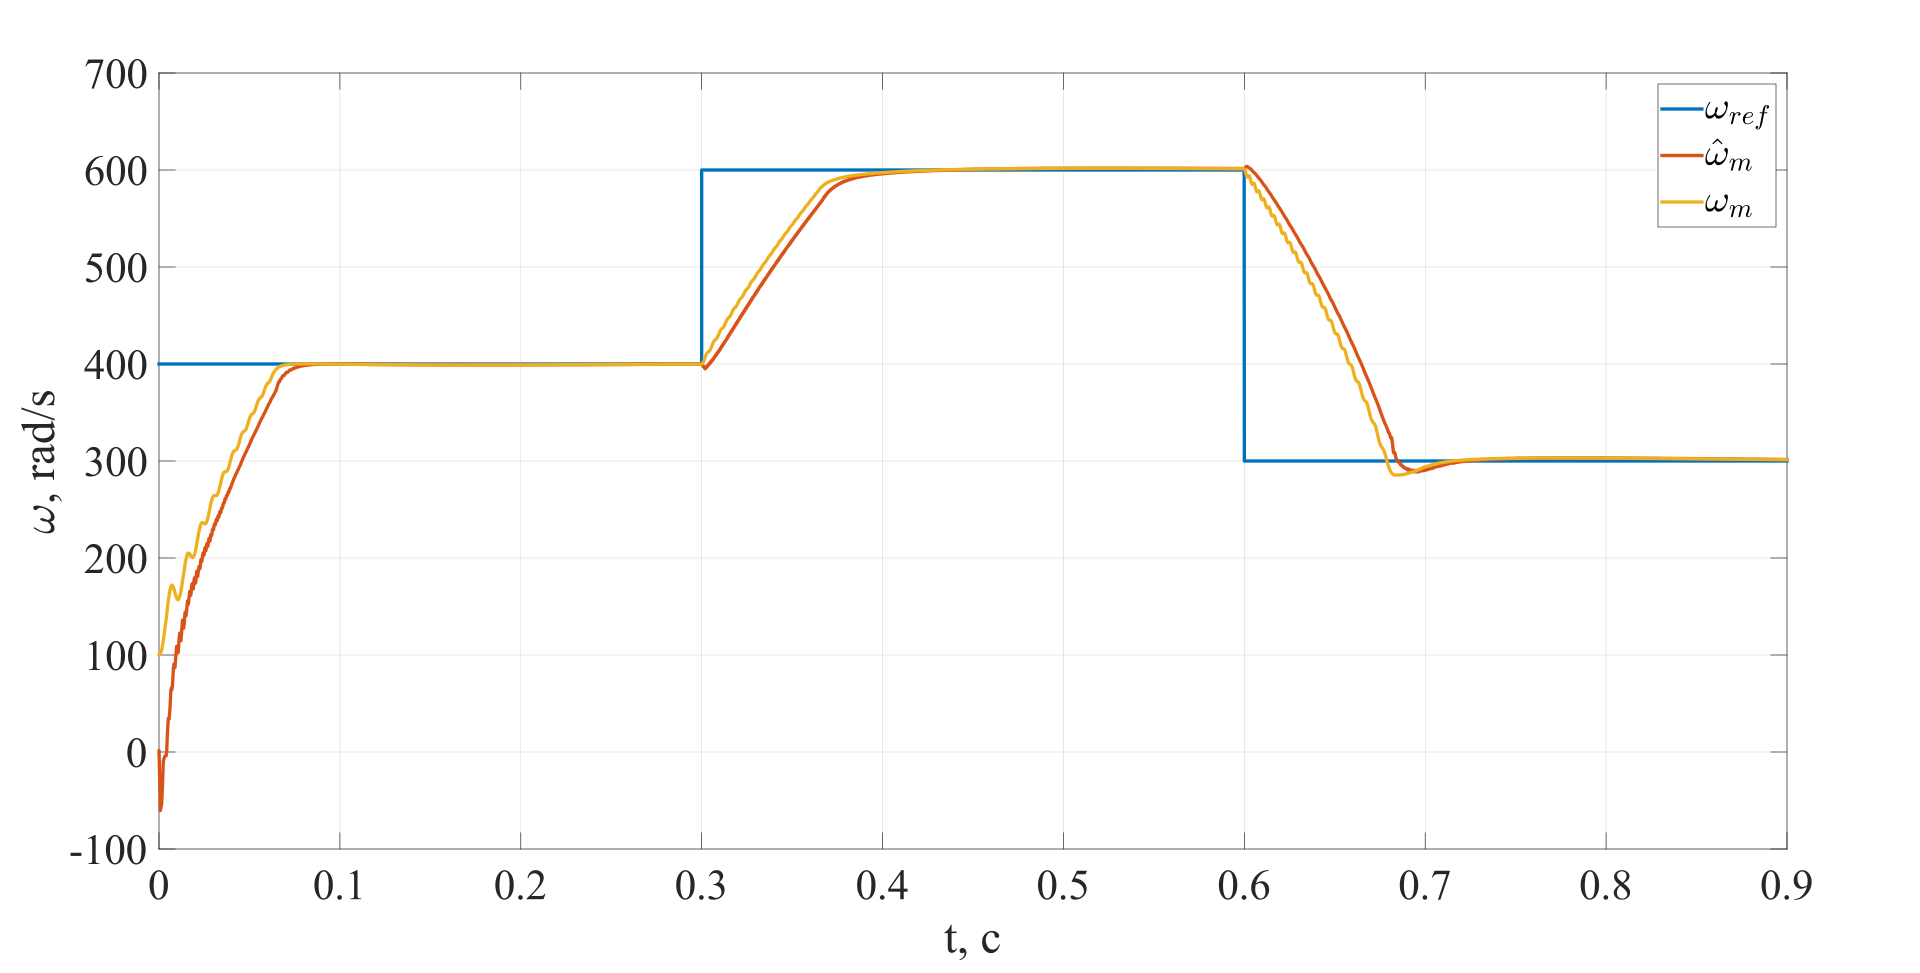
\includegraphics[width=\textwidth]{inc/svg/mod_resL+}
\caption{Заданная, оцененная и действительная скорость ротора при увеличении $L$ на $10$ \%}
\label{pic:L+}
\end{figure}

\begin{figure}[!h]
\centering
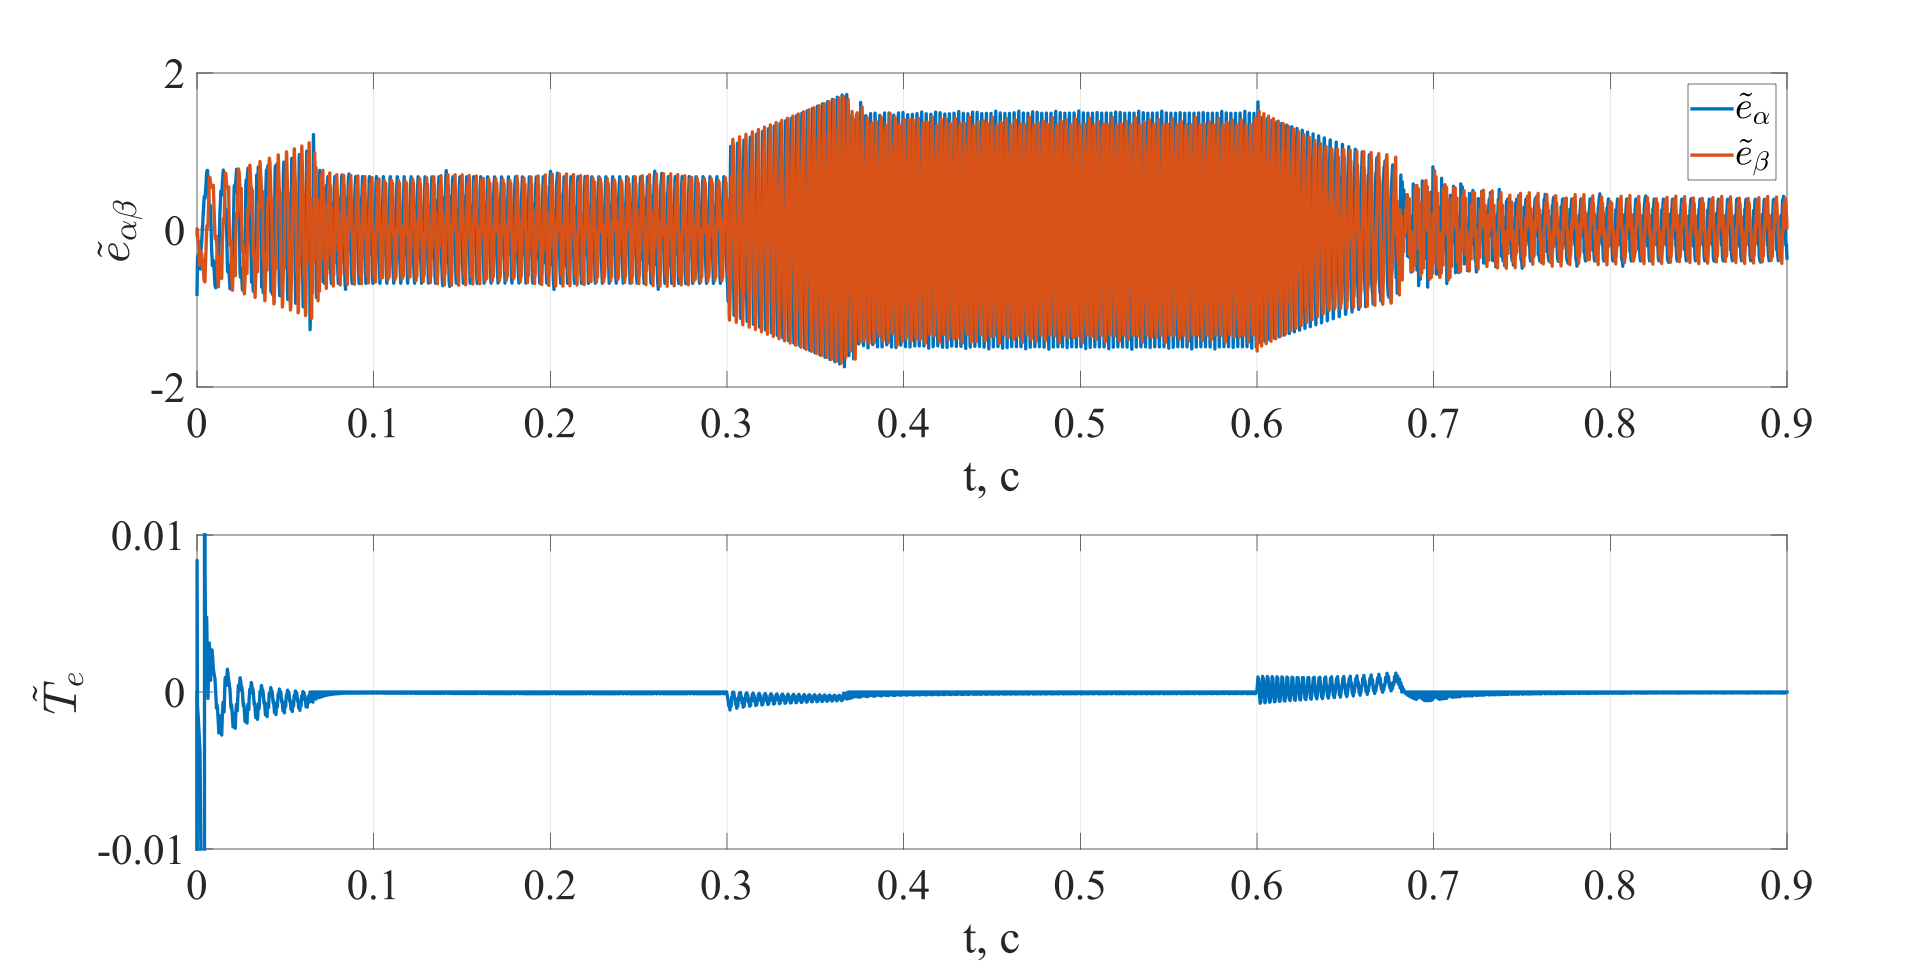
\includegraphics[width=\textwidth]{inc/svg/mod_res2L+}
\caption{Вектор невязки по противо-ЭДС и электромагнитному моменту при увеличении $L$ на $10$ \%}
\label{pic:2L+}
\end{figure}
